\documentclass[article]{report} % a4paper
% Some basic packages

\usepackage[utf8]{inputenc}
\usepackage[T1]{fontenc}
\usepackage{textcomp}
% Figure out whether you need this in English 
\usepackage[UKenglish]{babel}
\usepackage{url}
\usepackage{graphicx}
\usepackage{float}
\usepackage{booktabs}
\usepackage{enumitem}

% Don't indent paragraphs, leave some space between them
\usepackage{parskip}

% Hide page number when page is empty
\usepackage{emptypage}
\usepackage{subcaption}
\usepackage{multicol}
\usepackage{xcolor}

% Other font I sometimes use.
% \usepackage{cmbright}

% Math stuff
\usepackage{amsmath, amsfonts, mathtools, amsthm, amssymb}
% \usepackage{physics}
% Fancy script capitals
\usepackage{mathrsfs}
\usepackage{cancel}
% Bold math
\usepackage{bm}
% Some shortcuts
\newcommand\N{\ensuremath{\mathbb{N}}}
\newcommand\R{\ensuremath{\mathbb{R}}}
\newcommand\Z{\ensuremath{\mathbb{Z}}}
\renewcommand\O{\ensuremath{\emptyset}}
\newcommand\Q{\ensuremath{\mathbb{Q}}}
\newcommand\C{\ensuremath{\mathbb{C}}}
\newcommand\T{\ensuremath{\mathbb{T}}}
\newcommand\U{\ensuremath{\mathscr{U}}}
\newcommand\Y{\ensuremath{\mathscr{Y}}}
\newcommand\F{\ensuremath{\mathbb{F}}}

\newcommand{\norm}[1]{\left\lVert#1\right\rVert}
\let\newforall\forall
\renewcommand\forall{\;\newforall\;}
% Put x \to \infty below \lim
\let\svlim\lim\def\lim{\svlim\limits}

%Make implies and impliedby shorter
\let\implies\Rightarrow
\let\impliedby\Leftarrow
\let\iff\Leftrightarrow
\let\epsilon\varepsilon

% Add \contra symbol to denote contradiction
\usepackage{stmaryrd} % for \lightning
\newcommand\contra{\scalebox{1.5}{$\lightning$}}

% \let\phi\varphi

% Command for short corrections
% Usage: 1+1=\correct{3}{2}

\definecolor{correct}{HTML}{009900}
\newcommand\correct[2]{\ensuremath{\:}{\color{red}{#1}}\ensuremath{\to }{\color{correct}{#2}}\ensuremath{\:}}
\newcommand\green[1]{{\color{correct}{#1}}}

% horizontal rule
\newcommand\hr{
    \noindent\rule[0.5ex]{\linewidth}{0.5pt}
}

% hide parts
\newcommand\hide[1]{}

% si unitx
\usepackage{siunitx}
\sisetup{locale = FR}

% Environments
\makeatother
% For box around Definition, Theorem, \ldots
\usepackage{mdframed}
\mdfsetup{skipabove=1em,skipbelow=0em}
\theoremstyle{definition}
\newmdtheoremenv[nobreak=true]{consequence}{Consequence}
\newmdtheoremenv[nobreak=true]{theorem}{Theorem}
\newmdtheoremenv[nobreak=true]{lemma}{Lemma}
\newmdtheoremenv[nobreak=true]{definition}{Definition}
\newmdtheoremenv[nobreak=true]{prop}{Proposition}
\newmdtheoremenv[nobreak=true]{law}{Law}
\newmdtheoremenv[nobreak=true]{corollary}{Corollary}
\newmdtheoremenv{conclusion}{Conclusion}
\newmdtheoremenv{bonus}{Bonus}
\newtheorem*{notation}{Notation}
\newtheorem*{issue}{Issue}
\newtheorem*{terminology}{Terminology}
\newtheorem*{application}{Application}
\newtheorem*{example}{Example}
\newtheorem*{eg}{Example}
\newtheorem*{question}{Question}
\newtheorem*{previouslyseen}{As previously seen}
\newtheorem*{remark}{Remark}
\newtheorem*{problem}{Problem}
\newtheorem*{observe}{Observe}
\newtheorem*{property}{Property}
\newtheorem*{intuition}{Intuition}
\newtheorem*{fact}{Fact}
\newtheorem*{result}{Result}
\newtheorem*{punch}{Punchline}

% Fix some spacing
% http://tex.stackexchange.com/questions/22119/how-can-i-change-the-spacing-before-theorems-with-amsthm
\makeatletter
\def\thm@space@setup{%
  \thm@preskip=\parskip \thm@postskip=0pt
}

% \lecture starts a new lecture (les in dutch)
%
% Usage:
% \lecture{1}{di 12 feb 2019 16:00}{Inleiding}
%
% This adds a section heading with the number / title of the lecture and a
% margin paragraph with the date.

% I use \dateparts here to hide the year (2019). This way, I can easily parse
% the date of each lecture unambiguously while still having a human-friendly
% short format printed to the pdf.

\usepackage{xifthen}
\def\testdateparts#1{\dateparts#1\relax}
\def\dateparts#1 #2 #3 #4 #5\relax{
    \marginpar{\small\textsf{\mbox{#1 #2 #3 #5}}}
}

\def\@lecture{}%
\newcommand{\lecture}[3]{
    \ifthenelse{\isempty{#3}}{%
        \def\@lecture{Lecture #1}%
    }{%
        \def\@lecture{Lecture #1: #3}%
    }%
    \subsection*{\@lecture}
    \marginpar{\small\textsf{\mbox{#2}}}
}



% These are the fancy headers
\usepackage{fancyhdr}
\pagestyle{fancy}

% LE: left even
% RO: right odd
% CE, CO: center even, center odd
% My name for when I print my lecture notes to use for an open book exam.
% \fancyhead[LE,RO]{Joseph Grosso}

\fancyhead[RO,LE]{\@lecture} % Right odd,  Left even
\fancyhead[RE,LO]{}          % Right even, Left odd

\fancyfoot[RO,LE]{\thepage}  % Right odd,  Left even
\fancyfoot[RE,LO]{}          % Right even, Left odd
\fancyfoot[C]{\leftmark}     % Center

\makeatother




% Todonotes and inline notes in fancy boxes
\usepackage{todonotes}
\usepackage{tcolorbox}

% Make boxes breakable
\tcbuselibrary{breakable}

% Usage: 
% \begin{correction}
%     Lorem ipsum dolor sit amet, consetetur sadipscing elitr, sed diam nonumy eirmod
%     tempor invidunt ut labore et dolore magna aliquyam erat, sed diam voluptua. At
%     vero eos et accusam et justo duo dolores et ea rebum. Stet clita kasd gubergren,
%     no sea takimata sanctus est Lorem ipsum dolor sit amet.
% \end{correction}
\newenvironment{correction}{\begin{tcolorbox}[
    arc=0mm,
    colback=white,
    colframe=green!60!black,
    title=Correction,
    fonttitle=\sffamily,
    breakable
]}{\end{tcolorbox}}

% Note -- Same as 'correction' but color of box is different
\newenvironment{note}{\begin{tcolorbox}[
    arc=0mm,
    colback=white,
    colframe=white!60!black,
    title=Note,
    fonttitle=\sffamily,
    breakable
]}{\end{tcolorbox}}




% Figure support as explained in my blog post.
\usepackage{import}
\usepackage{xifthen}
\pdfminorversion=7
\usepackage{pdfpages}
\usepackage{transparent}
\newcommand{\incfig}[1]{%
    \def\svgwidth{\columnwidth}
    \import{./figures/}{#1.pdf_tex}
}

% Fix some stuff
% %http://tex.stackexchange.com/questions/76273/multiple-pdfs-with-page-group-included-in-a-single-page-warning
\pdfsuppresswarningpagegroup=1

% Remove leading zeroes from table of contents 
\renewcommand{\thesection}{\arabic{section}}

% My name
\author{Joseph Grosso}


\DeclareMathOperator{\length}{length}
\DeclareMathOperator{\Aut}{Aut}
\DeclareMathOperator{\diam}{diam}
\DeclareMathOperator*{\res}{res}
\title{Probability II}

\begin{document}
    \maketitle
    \tableofcontents
    % start lectures
    \lecture{1}{Mon 06 Jan 2020 08:30}{Syllabus}	
	\section{Syllabus}
	\begin{description}
		\item[Instructor] Glen Takahara - Jeffery Hall 407, phone \# 533-2430, Email: takahara@mast.queensu.ca
		\item[Assignments] There will be 9 homework assignments. These will be posted on the class web site; no paper copies will be handed out. Assignment 1 is due on Thursday, Jan. 23. Solutions to the assignments will be posted on the course web page. 
		\item[Resources] Under the resources tab there are a bunch of midterms and exams with solutions.
		\item[Grading] 20\% homework, 20\% mid-term test, 60\% final exam. 
		\item[Midterm Test] Scheduled for Thursday Feb 27 in class (9:30-10:30). 
	\end{description}

	\section{Part 1: Multiple Random Variables}
	2020-01-06 

	$S$ is the underlying sample space of a random variable. We can define a probability measure $P$ on $S$, which takes these events to number between 0 and 1, ie its probability. $P$ is defined on all "reasonable, well-behaved" subsets of S. 

	\[
		P : \text{"reasonable" subset of S} \to  [0, 1]
	.\] 
	

    \lecture{2}{Mon 13 Jan 2020 08:33}{}

    %\lecture{3}{Tue 21 Jan 2020 14:29}{Lab 3: Bode Plots}

\section{Introduction}
In this lab we learned about Bode plots and saw how their theoretical values corresponded with the real world outputs of our motor. 

\section{Deliverable}
\subsection{Bode Plots}
\begin{figure}[H]
	\centering
	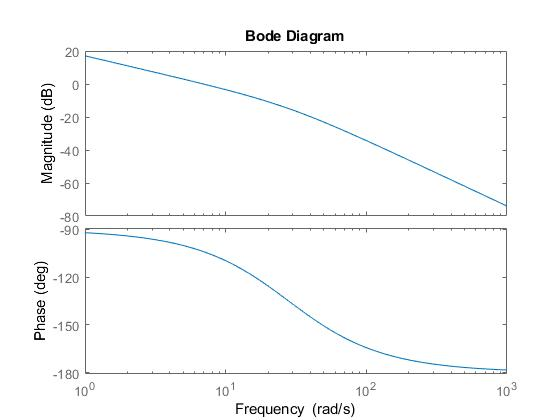
\includegraphics[width=0.8\textwidth]{./figures/lab2_theta.jpg}
	\caption{Bode plot for $\theta$ (Generated by MatLab)}
	\label{fig:}
\end{figure}

\begin{figure}[H]
	\centering
	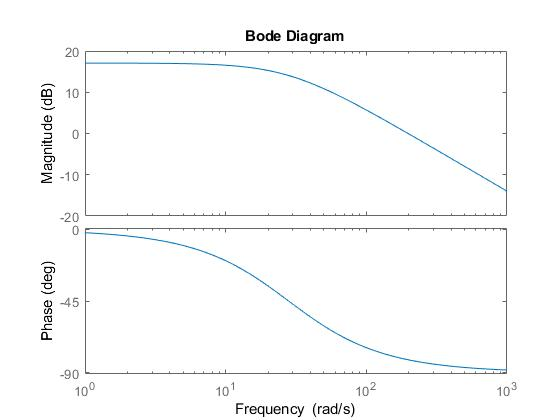
\includegraphics[width=0.8\textwidth]{./figures/lab2_omega.jpg}
	\caption{Bode plot for $\omega$ (Generated by MatLab)}
	\label{fig:}
\end{figure}

\section{Angular Position \& Velocity Plots}

\begin{figure}[H]
	\centering
	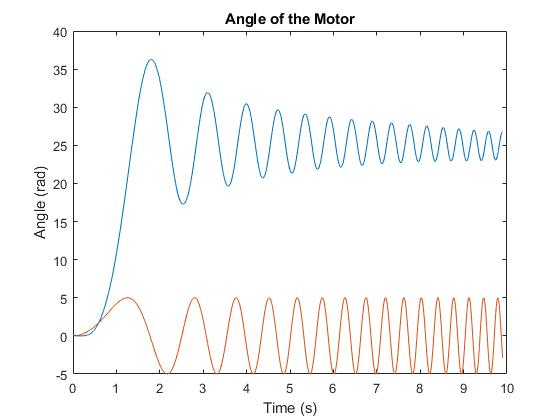
\includegraphics[width=0.8\textwidth]{./figures/lab2_theta_with_input.jpg}
	\caption{Motor Angular Position}
	\label{fig:}
\end{figure}

\begin{figure}[H]
	\centering
	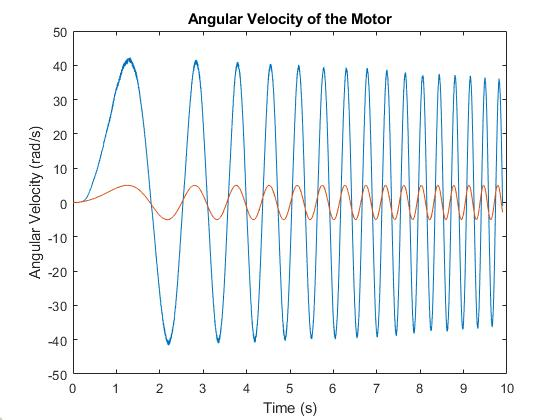
\includegraphics[width=0.8\textwidth]{./figures/lab2_omega_with_input.jpg}
	\caption{Motor Velocity}
	\label{fig:}
\end{figure}

For the plot of $\omega$, as the frequency increased, the amplitude stayed constant for a while and then began to slowly decrease, which matches the Bode plot. For the phase angle both sinusodes began at a phase angle of 0 degrees. As the frequency increased, the phase angle appears to decrease over time, but we could not quantify this difference because our test ended. 

For the plot of $\theta$, as frequency increased the amplitude decreased, which was predicted by the Bode plot. At very low frequencies, the amplitude tended towards very large values. The phase angle origin began at a trough, which signifies a phase angle of -90 degrees, while the other one began at a phase angle of 0, both predictions following along with our Bode plots.  

\subsection{Tabulated Data}

\begin{table}[H]
	\centering
	\caption{Data Collection Table}
	\label{tab:data-collection}
	\begin{tabular}{|| c c c c c c ||}
		\hline
		$\omega$ & Magnitude & Gain (dB) & Zero-Time Difference & Phase (rad) & Phase (deg) \\ [0.5ex]
		\hline\hline
		0.5 & 7.2805 & 17.2433 & 0.2364 & 0.1182 & -6.7726 \\
		\hline
		0.7896 & 6.9883 & 16.8875 & 0.0467 & 0.0368 & -2.1106 \\
		\hline 
		1.2469 & 7.037 & 16.3012 & -0.0597 & 0.0745 & 4.2661 \\
		\hline 
		1.9692 & 7.2075 & 17.1557 & 0.0183 & 0.0361 & -2.0663 \\
		\hline
		3.1098 & 6.9883 & 16.8875 & 0.0509 & 0.1582 & -9.0661 \\
		\hline
		4.911 & 6.8666 & 16.7348 & -0.0079 & -0.00386 & 2.2102 \\
		\hline 
		7.7554 & 6.5501 & 16.3249 & 0.0295 & 0.2285 & -13.0901 \\
		\hline 
		12.2474 & 5.99 & 15.5486 & 0.0317 & 0.3888 & -22.2763 \\
		\hline 
		19.3413 & 5.3813 & 14.6177 & 0.0268 & 0.5181 & -29.6827 \\
		\hline 
		30.5439 & 4.6751 & 13.3959 & 0.00206 & 0.6284 & -36.0026 \\
		\hline 
		48.2352 & 3.0924 & 9.8059 & 0.0174 & 0.841 & -48.1836 \\
		\hline 
		76.1734 & 3.0924 & 9.8059 & 0.0114 & 0.8668 & -49.6612 \\
		\hline 
		120.2936 & 2.3132 & 7.2843 & 0.0089 & 1.0757 & -61.6309 \\
		\hline 
		189.9696 & 1.7288 & 4.755 & 0.0077 & 1.4687 & -84.1504 \\
		\hline 
		300 & 1.534 & 3.7167 & 0.0068 & 2.0292 & -116.2648 \\
		\hline 
	\end{tabular}
\end{table}

\subsection{Experimental Bode Plots}

\begin{figure}[H]
	\centering
	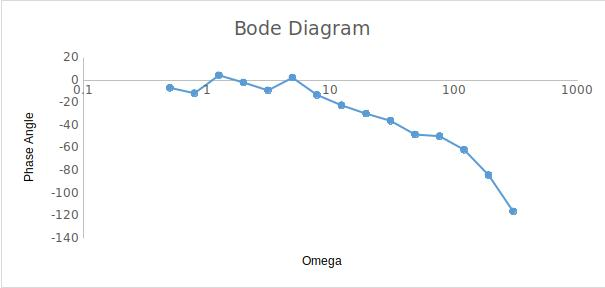
\includegraphics[width=0.8\textwidth]{./figures/lab2_experiment_phase.jpg}
	\caption{Experimental bode plot for phase angle}
	\label{fig:}
\end{figure}

\begin{figure}[H]
	\centering
	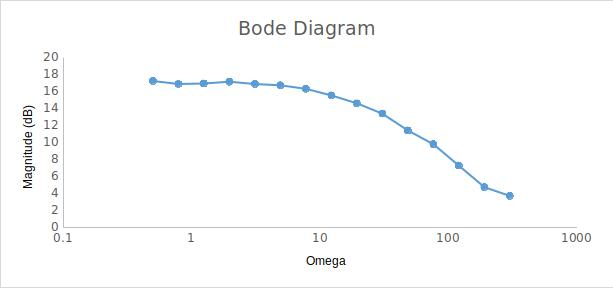
\includegraphics[width=0.8\textwidth]{./figures/lab2_experiment_magnitude.jpg}
	\caption{}
	\label{fig:}
\end{figure}

    % \lecture{4}{Tue 04 Feb 2020 14:30}{393 Lab 4}

\section{Plots of System response varying $\omega_{0}$, $\zeta$}
The result of varying $\zeta$ is the graph in Figure \ref{fig:varying-zeta}.
\begin{figure}[H]
	\centering
	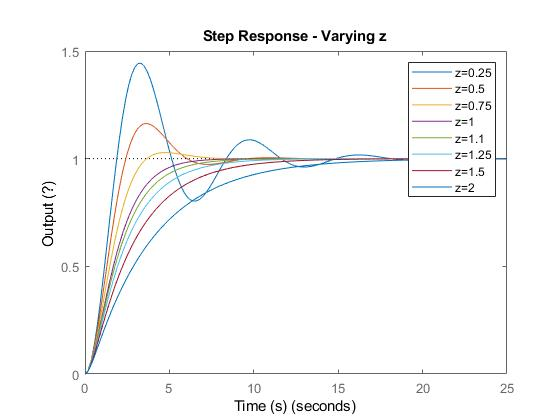
\includegraphics[width=0.8\textwidth]{./figures/lab4_fig1-part4-3-1-z.jpg}
	\caption{A plot of the system response when varying the value of $\zeta$}
	\label{fig:varying-zeta}
\end{figure}
As you can see an increase in $\zeta$ increases the damping of the output, where $\zeta=1$ seems to be close to the critical damping value, $\zeta < 1$ is an underdamped system and $\zeta > 1$ is an overdamped system. 

The result of varying $\omega_{0}$ is seen in Figure \ref{fig:varying-w0}.
\begin{figure}[H]
	\centering
	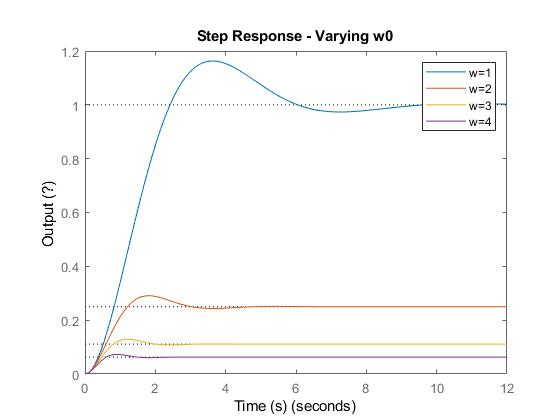
\includegraphics[width=0.8\textwidth]{./figures/lab4_fig2-part4-3-1-w0.jpg}
	\caption{A plot of the system response when varying the value of $\omega _{0}$}
	\label{fig:varying-w0}
\end{figure}
The greater the value of $\omega_{0}$, the smaller the steady-state value of the system. 

\section{Effects of Changing $\alpha$}  %Maxym
For positive values of $\alpha$, the effect of increasing $\alpha$ is the graph in Figure \ref{fig:varying-alpha-positive}.
\begin{figure}[H]
	\centering
	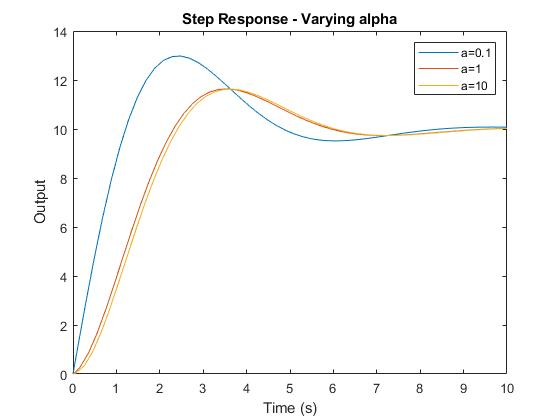
\includegraphics[width=0.8\textwidth]{./figures/lab4_fig3-part4-3-2-positive.jpg}
	\caption{A plot of the system response when varying the positive values of $\alpha$}
	\label{fig:varying-alpha-positive}
\end{figure}
As $\alpha$ increases, the rise time of the system also increases. While there is a large difference between the rise times of $\alpha = 0.1$ and $\alpha = 1$, the difference between $\alpha = 1$ and $\alpha = 10$ is relatively small. Meanwhile, settling time for all positive values of $\alpha$ appear relatively similar with all of the values converging to 10 at approximately 10 seconds. All three positive values of $\alpha$ displayed overshoot with $\alpha = 0.1$ having the largest overshoot while $\alpha =1$ and $\alpha = 10$ had smaller overshoots. Similarly, the peak time of $\alpha = 0.1$ is much shorter than the peak times of $\alpha = 1$ and $\alpha = 10$. The graph shows that $\alpha = 10$ has the longest peak time. 

For negative values of $\alpha$, the effect of increasing $\alpha$ is the graph in Figure \ref{fig:varying-alpha-negative}.
\begin{figure}[H]
	\centering
	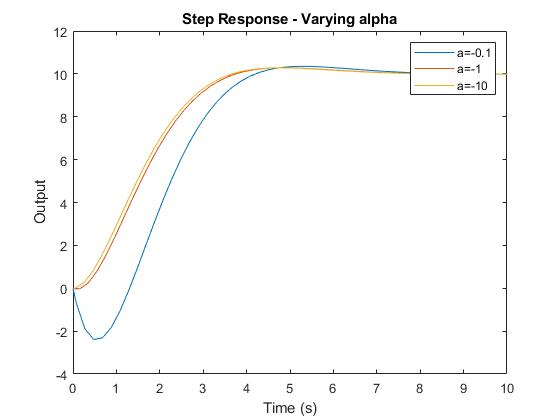
\includegraphics[width=0.8\textwidth]{./figures/lab4_fig4-part4-3-2-negative.jpg}
	\caption{A plot of the system response when varying the negative value of $\alpha$}
	\label{fig:varying-alpha-negative}
\end{figure}
As $\alpha$ increases negatively, the rise time of the system decreases. While there is a large difference between the rise times of $\alpha = -0.1$ and $\alpha = -1$, the difference between $\alpha = -1$ and $\alpha = -10$ is relatively small. Meanwhile, settling time for all negative values of $\alpha$ appear relatively similar with all of the values converging to 10 at just under 10 seconds. All three negative values of $\alpha$ displayed small overshoot with $\alpha = -0.1$ having a slightly larger overshoot than $\alpha =1$ and $\alpha = 10$. The peak time of $\alpha = -0.1$ is slightly longer than the peak times of $\alpha = 1$ and $\alpha = 10$ which had similar peak times.
% End Maxym Section

\section{Why Are The Plots The Same?}
\begin{figure}[H]
        \centering
        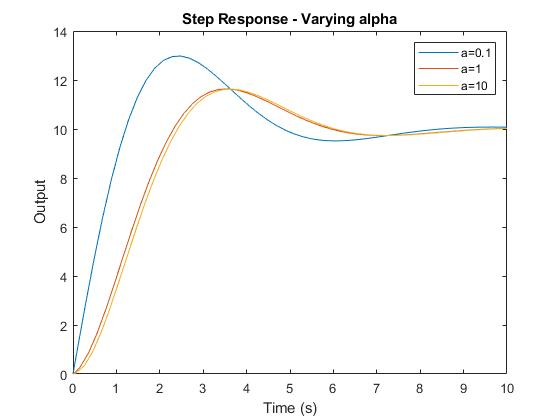
\includegraphics[width=0.8\textwidth]{./figures/lab4_fig3-part4-3-2-positive.jpg} % Put the plots in the figures sub     directory
        \caption{A one-sentence description of the plot or figure}
        \label{fig:name} % basically a variable name you can refer to in the text 
\end{figure}

\begin{figure}[H]
        \centering
        \includegraphics[width=0.8\textwidth]{./figures/lab4_fig3-part4-3-2-negative.jpg} % Put the plots in the figures sub     directory
        \caption{A one-sentence description of the plot or figure}
        \label{fig:name} % basically a variable name you can refer to in the text 
\end{figure}

\section{System Type Section}

\begin{table}[h]
\begin{tabular}{|l|l|l|l|l|}
System & \begin{tabular}[c]{@{}l@{}}Response to \\ Constant Input\end{tabular}                    & \begin{tabular}[c]{@{}l@{}}Response to \\ Linear Input\end{tabular}                      & \begin{tabular}[c]{@{}l@{}}Response to \\ Quadratic Input\end{tabular}                  & Type \\ \hline
1      & \begin{tabular}[c]{@{}l@{}}Settling Time 0.4s\\ Steady Error \textless 0.01\end{tabular} & \begin{tabular}[c]{@{}l@{}}Settling Time 0.4s\\ Steady Error \textless 0.08\end{tabular} & \begin{tabular}[c]{@{}l@{}}Settling Time 0.4s\\ Steady Error \textless 0.1\end{tabular} & 1    \\
2      & \begin{tabular}[c]{@{}l@{}}No Steady State\\ Error was Sinusoidal\end{tabular}           & \begin{tabular}[c]{@{}l@{}}No Steady State\\ Error was Sinusoidal\end{tabular}           & \begin{tabular}[c]{@{}l@{}}No Steady State\\ Error was Sinusoidal\end{tabular}          & 0    \\
3      & \begin{tabular}[c]{@{}l@{}}Settling Time 0.7s\\ Steady Error 8.5\end{tabular}            & \begin{tabular}[c]{@{}l@{}}No Steady State\\ Error was Linear\end{tabular}               & \begin{tabular}[c]{@{}l@{}}No Steady State\\ Error was Quadratic\end{tabular}           & 0
\end{tabular}
\end{table}

With a proportional control of \(P = 5\), the response tracked constant input \ref{fig:system1_constant}, linear input \ref{fig:system1_linear}, and constant input \ref{fig:system1_quadratic} all with a rise time of approximately \(0.4 s\) and steady state error of \(< 0.1\) in all cases. However, in the case of linear and quadratic input, the signal did not stabilize within a small error margin of the input signal and the error was not steady, which matches with the prediction that this is a type 1 system.

With a integral control of \(I = 1\), the response did not track any input, and the error was sinusoidal and increasing, or not BIBO stable in all cases. The response is graphed in the constant case \ref{fig:system2_constant}, linear \ref{fig:system2_linear}, and quadratic \ref{fig:system2_quadratic} This aligns with our predictions that System 2 is a Type 0 system.

With a derivative control of \(D = 1\), the response reached a steady state response with constant input \ref{fig:system3_constant}, but with a very large steady state error of \(8.5\) after \(0.7 s\). In the linear \ref{fig:system3_linear} and quadratic \ref{fig:system3_quadratic} cases, the steady state error was linear and quadratic respectively, and increasing. No steady state was reached, and the constant steady state was not acceptable, which agrees with our predictions that System 3 is a Type 0 system.

\begin{figure}[H]
        \centering
        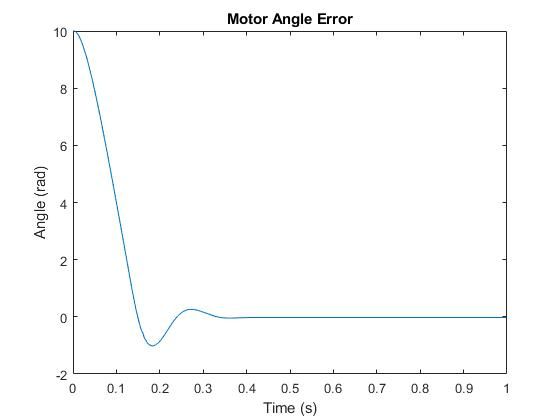
\includegraphics[width=0.8\textwidth]{./figures/lab4_fig7-part4-3-3-error-rc5.jpg}
        \caption{System 1 Response to Constant Input}
        \label{fig:system1_constant}
\end{figure}

\begin{figure}[H]
        \centering
        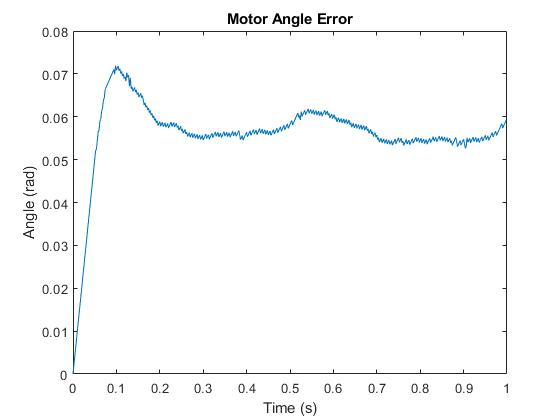
\includegraphics[width=0.8\textwidth]{./figures/lab4_fig8-part4-3-3-error-rc5-linear.jpg}
        \caption{System 1 Response to Linear Input}
        \label{fig:system1_linear}
\end{figure}

\begin{figure}[H]
        \centering
        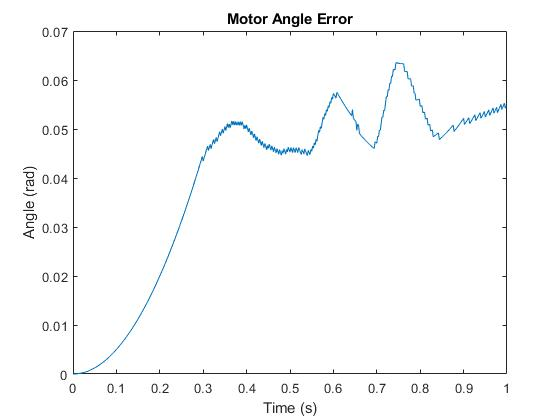
\includegraphics[width=0.8\textwidth]{./figures/lab4_fig9-part4-3-3-error-rc5-quadratic.jpg}
        \caption{System 1 Response to Quadratic Input}
        \label{fig:system1_quadratic}
\end{figure}

\begin{figure}[H]
        \centering
        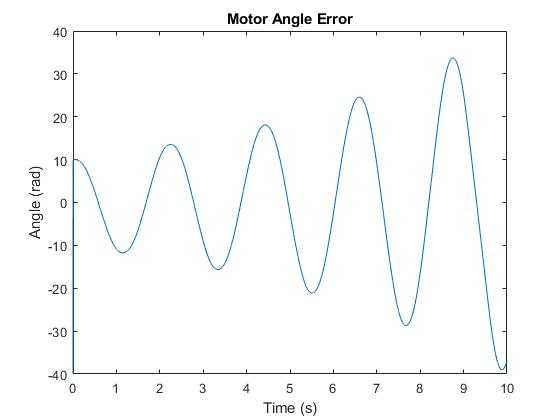
\includegraphics[width=0.8\textwidth]{./figures/lab4_fig10-part4-3-3-error-rc-I=1-constant.jpg}
        \caption{System 2 Response to Constant Input}
        \label{fig:system2_constant}
\end{figure}

\begin{figure}[H]
        \centering
        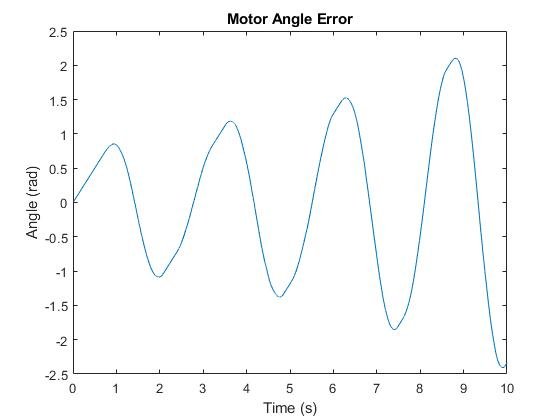
\includegraphics[width=0.8\textwidth]{./figures/lab4_fig11-part4-3-3-error-rc-I=1-linear.jpg}
        \caption{System 2 Response to Linear Input}
        \label{fig:system2_linear}
\end{figure}

\begin{figure}[H]
        \centering
        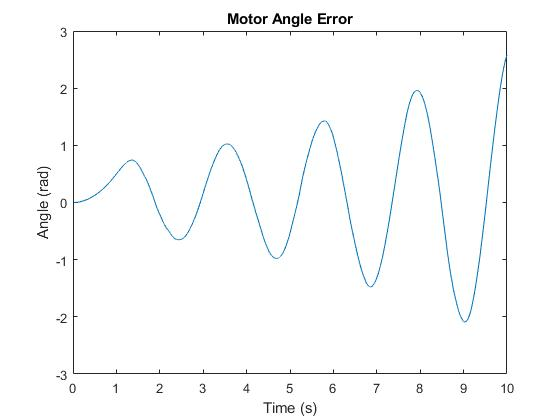
\includegraphics[width=0.8\textwidth]{./figures/lab4_fig12-part4-3-3-error-rc-I=1-quadratic.jpg}
        \caption{System 2 Response to Quadratic Input}
        \label{fig:system2_quadratic}
\end{figure}

\begin{figure}[H]
        \centering
        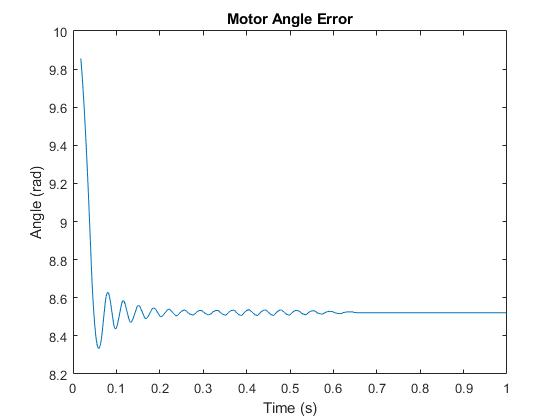
\includegraphics[width=0.8\textwidth]{./figures/lab4_fig13-part4-3-3-error-rc-D=1-constant.jpg}
        \caption{System 3 Response to Constant Input}
        \label{fig:system3_constant}
\end{figure}

\begin{figure}[H]
        \centering
        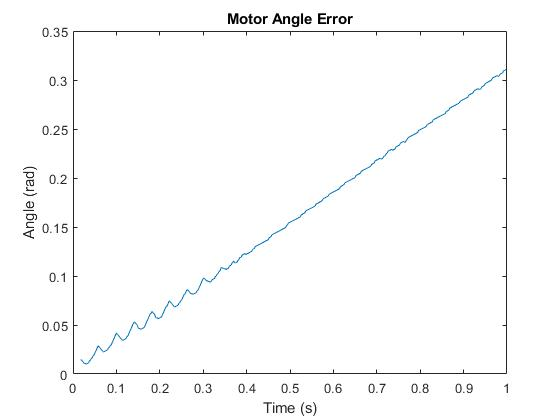
\includegraphics[width=0.8\textwidth]{./figures/lab4_fig14-part4-3-3-error-rc-D=1-linear.jpg}
        \caption{System 3 Response to Linear Input}
        \label{fig:system3_linear}
\end{figure}

\begin{figure}[H]
        \centering
        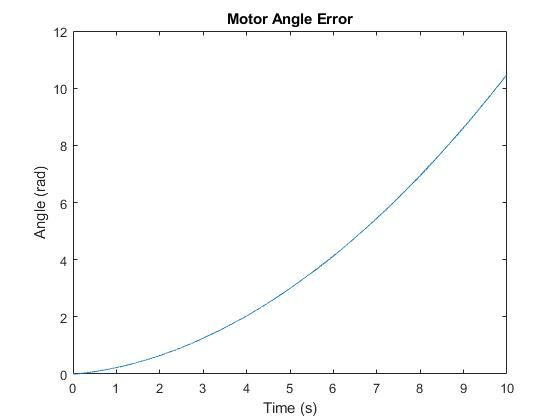
\includegraphics[width=0.8\textwidth]{./figures/lab4_fig15-part4-3-3-error-rc-D=1-quadratic.jpg}
        \caption{System 3 Response to Quadratic Input}
        \label{fig:system3_quadratic}
\end{figure}

    \lecture{5}{Tue 14 Jan 2020 10:26}{Addendum to guest lecture}

\begin{remark}[Limits of $x_{i}$ in the Multivariate Hypergeometric distribution]
	The constraints that Michael (guest lecturer) wrote are: 
	\begin{align*}
		x_1 + \ldots+ x_{r} &=  k \\
		max(0, k - \left( N - n_i \right) ) &\le x_{i} \le min\left( n_{i}, k \right) \\
		i &= 1, \ldots, r
	.\end{align*}
	There is an additional constraint: $x_{i} $ is an integer, $i = 1, \ldots, r$.

	Alternatively, we can set the constraints to be 
	\begin{align*}
		x_1 + \ldots + x_r &= k \\
		x_{i} &\in  \left\{ 0, 1, \ldots, n_{i} \right\} , i = 1, \ldots, r
	.\end{align*}
\end{remark}

An alternative way to describe the distribution of $\left( X_1, \ldots, X_{r} \right) $ is to describe the distribution of $\left( X_1, \ldots, X_{r-1} \right) $ and use the constraint $X_1 + \ldots + X_{r} = k$. 

We have:
\begin{align*}
	P\left( X_1 = x_1, \ldots, X_{r-1} = x_{r-1} \right) &= P\left( X_1= x_1, \ldots, 
	X_{r-1} = x_{r-1}, X_r = k - x_1-\ldots-x_{r-1} \right)  \\
							     &=\frac{\binom{n_1}{x_1} \binom{n_2}{x_2} \cdots \binom{n_{r-1}}{x_{r-1}}  \binom{n_{r}}{k-x_1-\ldots-x_{r-1}}}{\binom{N}{k}}
.\end{align*}
for:
\begin{align*}
	0 &\le x_1 + \ldots + x_{r-1} \le k \\
	x_i &= 0, \ldots, n_{i} \\
	max&\left( 0, k-\left( N - n_{i} \right)  \right) \le x_{i}\\
	i &= 1, \ldots, r-1 
.\end{align*}
We can write the marginal distribution of $\left( X_{i_{i}}, \ldots, X_{i_{d}} \right) $, $\left\{ i_{1}, \ldots, i_{d} \right\}  \subset \left\{ 1, \ldots, r \right\} $ by relabelling the objects in the population as types $i_{1}, \ldots, i_{d}$,and "other". 

There are $N - n_{i_{1}} - \ldots - n_{i_{d}}$ objects of type other.

Using the second version of the Multivariate Hypergeometric distribution, we have that the joint pmf of $\left( X_{i_{1}}, \ldots, X_{i_{d}} \right) $ is 
\begin{align*}
	P\left( X_{i_{1}}= x_{i_{1}}, \ldots, X_{i_{d}} = x_{i_{d}} \right) 
	&= \frac{\binom{n_{i_{1}}}{x_{i_{1}}}  \cdots \binom{n_{i_{d}}}{x_{i_{d}}}  \binom{N - n_{i_{1}} - \ldots - n _{i_{d}}}{k-x_{i_{1}}-\ldots-x_{i_{d}}}}{\binom{N}{k}}
 \\
	0 \le x_{i_{1}} + \ldots + x_{i_{d}} &\le  k \quad x_{ij} = 0, \ldots, n_{i_{j}}\\
	max\left( 0, k- \left( N - n_{ij} \right)  \right) &\le x_{ij}, \quad j = 1, \ldots, d
.\end{align*}

    \lecture{6}{Fri 17 Jan 2020 15:55}{}

Last time: $\hat{F} : \T \times X  \to \R^{n}$ 

Solution: $\dot{\xi} \left( t \right) = \hat{F}\left( t, \xi \left( t \right)  \right) $, almost everywhere $t \in  \T' \subseteq \T$. 

Domain:
\[
D_{\hat{F}} = \left\{ \left( t, t_0, x_0 \right) \in \T\times \T\times X \\
\mid \text{ solution exists at time }t, w \text{ initial conclusion }x_0 \text{ at initial time } t_0\right\} 
.\] 

Flow: $\Phi ^{\hat{F}} : D_{\hat{F}} \to X$ satisfies 
\[
	\frac{d}{dt}\Phi ^{\hat{F}}\left( t, t_0, x_0 \right)  = \hat{F}\left( t, \Phi ^{\hat{F}}\left( t, t_0, x_0 \right)  \right) , \quad \Phi ^{\hat{F}}\left( t_0, t_0, x_0 \right)  = x_0
.\] 
\begin{example}
	$\T = \R$, $X = \R$, $\hat{F}\left( t, x \right) = x^2$. Solution with initial condition $x_0$ at time $t_0$ satisfies 
	\begin{align*}
		\dot{\xi }\left( t \right)  &=  \xi \left( t \right) ^2 \\
		\xi \left( t_0 \right) &= x_0 \\
		\dot{x} &= x^2 \\
		\frac{dx}{x^2} &= dt \\
		\implies x\left( t \right) &= \frac{x_0}{1 - x_0\left( t - t_0 \right) } 
	.\end{align*}

	\[
		D_{\hat{F}} = \left\{ \left( t, t_0, x_0 \right)  \mid \begin{cases}
				t \in \left( -\infty, t_0 + \frac{1}{x_0} \right) & x_0 > 0 \\
				t \in  \left( t_0 + \frac{1}{x_0}, \infty \right) & x_0 < 0 \\
				t \in  \left( -\infty, \infty \right)  & x = 0
		\end{cases} \right\} 
	.\] 
	\begin{align*}
		\Phi ^{\hat{F}}: D_{\hat{F}} &\longrightarrow \R \\
		\left( t, t_0, x_0 \right)  &\longmapsto \Phi ^{\hat{F}}(\left( t, t_0, x_0 \right) ) = \frac{x_0}{1 - x_0\left( t - t_0 \right) }
	.\end{align*}
\end{example}

For linear equations, there are no restrictions on the times for which solutions exist.
\[
\implies D_{\hat{F}} = \T \times  \T \times  X 
.\] 

\subsection{Autonomous ODE's (independent of time)}

An ODE $\hat{F} : \T \times  R  \to \R ^{n} $ is autonomous if $\exists  \hat{F}_{0} : X  \to \R^{n}$ so that $\hat{F}\left( t, x \right) = \hat{F} _{0}\left( x \right) $. This just captures the idea of independence of time. 

    \lecture{7}{Mon 20 Jan 2020 08:39}{Marginal CDF's}

\begin{definition}
	Let $X_1, \ldots, X_{n}$ have joint cdf $F_{x}\left( x_1, \ldots, x_{n} \right)  = P \left( X_{1} \le x_1, \ldots, X_{n}\le x_{n} \right) $. 

	Let $\left\{ i_1, \ldots, i_{k} \right\} \subset \left\{ 1,\ldots,n \right\} $ and 
	\[
	\left\{ j_1, \ldots, j_{n-k} \right\} = \left\{ 1, \ldots, n \right\} \ \left\{ i_1, \ldots, i_{k} \right\} 
	.\] 
	where $i_1, \ldots, i_{k}$ are distinct. 

	The joint marginal CDF of  $\left( X_{i_1} ,\ldots, X_{i_{k}} \right) $ is 
	\begin{align*}
		F_{X_{i_1}, \ldots, X_{i_{k}}}\left( x_{i_{1}}, \ldots, x_{i_{k}} \right) 
		&= P\left( X_{i_{1}} \le  x_{i_{1}}, \ldots, X_{i_{k}} \le  x _{i_{k}} \right) \\ 
		&= P\left( X_{i_{1}} \le  x_{i_{i}} ,\ldots, X_{i_{k}} \le X_{i_{k}} \le x_{i_{k}}, \
		X_{j_{1}} < \infty, \ldots, X _{j_{n-k}} < \infty \right)  \\
	        &=  \lim_{x_{j_{1}} \to \infty, \ldots , x_{j_{n - k}} \to \infty} P\left( X_{i_{1}} \le  x_{i_{i}} ,\ldots, X_{i_{k}} \le X_{i_{k}} \le x_{i_{k}}, X_{j_{1}} < \infty, \ldots, X _{j_{n-k}} < \infty \right) 
	.\end{align*}

	In other words, take the full joint CDF and let elements $j_1, \ldots, j_{n - k} \to \infty$. 
\end{definition}

\section{Independence of Multiple Random Variables}

First, let us look at $n$ events $A_1, \ldots, A_{n}$. What do we mean for them to be mutually independent?

For $n = 2$: Intuitively (and mathematically), we want $P\left( A_1  \mid A_2\right) = P\left( A_1 \right) $ where $P\left( A_1 \mid A_2 \right) $ is the conditional probability of $A_1$ given $A_2$. 

\begin{figure}[ht]
    \centering
    \incfig{venn-diagram-of-$-and-$}
    \caption{Venn Diagram of $A_{1}$ and $A_2$}
    \label{fig:venn-diagram-of-$-and-$ }
\end{figure}

In the new probability space above, the crossed lines implies that $A_1$ happened given $A_2$ occurred. Then
 \[
	 P\left( A_1 \mid A_2 \right)  = \frac{P\left( A_1 \cap A_2 \right) }{P\left( A_2 \right) }
.\]
So if $A_1$ and $A_2$ are independent, then we have 
\begin{align*}
	\frac{P\left( A_1 \cap A_2 \right) }{P\left( A_2 \right) } &= P\left( A_1 \right)  \\
	\implies P\left( A_1 \cap A_2 \right)  &= P\left( A_1 \right) P\left(A_2 \right) 
.\end{align*}

Now consider n events $A_1, \ldots, A_n$.

\begin{definition}
	$A_1, \ldots, A_{n}$ are mutually independent if 
	\begin{align*}
		P\left( A_1\cap \ldots \cap A_{n} \right) &= P\left( A_1 \right) \times \ldots \times P\left( A_{n} \right) \\
	P\left( A_{i_{1}}\cap \ldots\cap A_{i_{k}}\right)  &= P\left( A_{i_1} \right) \times  \ldots \times  P\left( A_{i_{k}} \right) \quad \forall \left\{i_1,\ldots, i_{k} \right\} \subset  \left\{ 1, \ldots, n \right\} 
	.\end{align*}
\end{definition}
\begin{remark}
	Pairwise independence $\not\implies$  mutual independence. 
	\begin{example}
		Three 
	\end{example}
\end{remark}

    \lecture{8}{Tue 21 Jan 2020 10:35}{Independence of Random Variables}

\begin{definition}
	We say that $n$ random variables $X_{1} , \ldots , X_{n}$ are mutually independent if 
	\[
		P\left( X_1 \in A_1, \ldots, X_{n} \in  A_{n} \right) = P\left( X_1 \in  A_1 \right) \times \ldots\times P\left( X_{n}\in A_{n} \right) 
	.\] 
	for any $A_{1} , \ldots , A_{n} \subset \R$ (any reasonable set).

	Note that we can take any of the $A_{i}$ to be $\R$, so if we take $\left\{ i_{1} , \ldots , i_{k} \right\} \subset \left\{ 1, \ldots , n \right\} $ and $\left\{ j_{1} , \ldots , j_{n-k} \right\}  = \left\{ 1, \ldots, n \right\}  \ \left\{ i_{1} , \ldots , i_{k} \right\} $ , then
	\begin{align*}
		P\left( X_{i_{j}} \in A_{i_{1}}, \ldots, X_{i_{k}} \in  A_{i_{k}} \right) &= P\left( X_{i_{1}} \in  A_{i_1}, \ldots, X_{i_{k}} \in A_{i_{k}}, X_{j_1} \in  A_{j_1} \in  \R, \ldots, X_{j_{n-k}} \in \R \right)  \\
											  &= P\left( X_{i_1} \in A_{i_1} \right) \ldots P\left( X_{i_{k}} \in  A_{i_{k}} \right) \left( 1 \right) \ldots \left( 1 \right)  \\
											  &= P\left( X_{i_1} \in A_{i_1} \right) \ldots P\left( X_{i_{k}} \in  A_{i_{k}} \right) 
	.\end{align*}
	So any subset of $X_{1} , \ldots , X_{n}$ are mutually independent if $X_{1} , \ldots , X_{n}$ are mutually independent. 
\end{definition}

\begin{remark}
	 \begin{enumerate}
		 \item If $X_{1} , \ldots , X_{n}$ are mutually independent then so are $g_{i}\left( X_1	 \right) , \ldots , g_{n}\left( X_{n} \right) $ where $g_{i} : \R \to \R, i = 1, \ldots, n$.
		 \item The $X^{ir}_{i}$ in the definition of independence can be any random quantities (eg, random vectors or random matrices). The only change is that the $A^{is}_{i}$ must be in the appropriate range space of $X_{i}$. 
	\end{enumerate}
\end{remark}

\begin{theorem}
	$X_{1} , \ldots , X_{n}$ are mutually independent if and only if $f_{x}\left( x_{1} , \ldots , x_{n} \right) = f_{X_{1}}\left( x_1 \right) \times  \ldots\times f_{X_{n}}\left( x_{n} \right) $ (cts case with marginal pdfs) or 
	 \[
		 P_{X}\left( x_{1} , \ldots , x_{n} \right) = P_{X_{1}}\left( x_1 \right) \times \ldots\times P_{X_{n}}\left( x_{n} \right) 
	.\] 
	(discrete case with marginal pmfs).

\begin{proof}
	Suppose the above factoring holds. Let $A_{1} , \ldots , A_{n}\subset \R$ be arbitrary. Then
	\begin{align*}
		P\left( X_1 \in  A_1, \ldots, X_{n} \in  A_{n} \right) &= \begin{cases}
			\int_{A_{n}}^{ } \ldots \int_{A_1}^{ } dx_{1} , \ldots , dx_{n}  & \text{continuous} \\
			\sum_{X_{n} \in  A_{n}}^{ } \ldots \sum_{x_1 \in  A_{n}}^{ }  P_{X}\left( x_{1} , \ldots , x_{n} \right) & \text{discrete}
		\end{cases}\\
		&= \begin{cases}
			\left( \int_{A_{n}}^{ } f_{X_{n}}\left(x_{n}\right) dx_{n} \right) 	\times \ldots\times \left( \int_{A_{1}}^{ } f_{X_{1}}\left(x_{1}\right) dx_{n} \right) \\
			\left( \sum_{x_{n} \in  A_{N}}^{ } P_{X_{n}}\left( x_{n} \right)  \right) \times  \ldots \times \left( \sum_{x_1 \in  A_1}^{ } P_{X_1}\left( x_1 \right)  \right) 
		\end{cases} \\
		&= P\left( X_{n} \in  A_{n} \right) \times \ldots\times P\left( X_1 \in  A_1 \right) 
	.\end{align*}
	Now assume that $X_{1} , \ldots , X_{n}$ are mutually independent:
	\begin{description}
		\item[Discrete Case] By independence
			\begin{align*}
				P\left( X_{1} = x_1, \ldots, X_{n} = x_{n}\right) &= P\left( X_1 = x_1 \right) \times \ldots\times P\left( X_{n} = x_{n} \right)  \\
				\implies P_{X}\left( x_{1} , \ldots , x_{n} \right) &= P_{X_1}\left( x_1 \right) \times \ldots\times P_{X_{n}}\left( x_{n} \right) 
			.\end{align*}
	\end{description}
\end{proof}
\end{theorem}

    \lecture{9}{Thu 23 Jan 2020 09:36}{Expectation and Multiple RVs}

\begin{theorem}
	$X_{1} , \ldots , X_{n}$ are mutually independent if and only if  
	\[
		F_X \left( x_{1} , \ldots , x_{n} \right) = F_{X_1} \left( x_1 \right) \times \ldots \times F_{X_{n}} \left( x_{n} \right) 
	.\] 
	where $F_{X}$ is joint cdf and $F_{X_{i}}$ is marginal cdf of $X_{i}$, $i = 1, \ldots, n$. 
	\begin{proof}
		Suppose $X_{1} , \ldots , X_{n}$are mutually independent. Then
		\begin{align*}
			F_{X}\left( x_{1} , \ldots , x_{n} \right) 
			&= P\left( X_1 \le x_1, \ldots, X_{n} \le  x_{n} \right)  \\
			&= P\left( X_1 \le x_1 \right)  \times \ldots\times  P\left( X_{n} \le x_{n} \right)  \\
			&= F_{X_1} \left( x_1 \right) \times \ldots\times F_{X_{n}}\left( x_{n} \right) 			
		.\end{align*}
		Now suppose that 
		\begin{align*}
			F_{X}\left( x_{1} , \ldots , x_{n} \right) &= F_{X_1} \left( x_1 \right) \times \ldots\times F_{X_{n}}\left( x_{n} \right) \quad \forall \left( x_{1} , \ldots , x_{n} \right) \in R^{n}
		.\end{align*}
		In this case when $X_{1} , \ldots , X_{n}$ are jointly continuous then from proof of previous theorem we get that $f_{X}\left( x_{1} , \ldots , x_{n} \right) = f_{X_1}\left( x_1 \right) \times \ldots\times f_{X_{n}}\left( x_{n} \right) $, which then implies that $X_{1} , \ldots , X_{n}$ are mutually independent.  
		
To prove that $F_{X}\left( x_{1} , \ldots , x_{n} \right) = F_{X_1}\left( x_1 \right) \times \ldots \times F_{X_{n}}\left( x_{n} \right) $ implies that $X_{1} , \ldots , X_{n}$ are mutually independent is outside of the scope of this course. 
	\end{proof}
\end{theorem}

\section{Expectation Involving Multiple Random Variables}

Expectation is only defined for random variables. If $X = \left( X_{1} , \ldots , X_{n} \right) ^{T}$ is a random vector then we may write $E\left[ X \right] $, which only means
\[
\begin{bmatrix} E\left[ X_1 \right] \\ \vdots\\ E\left[ X_n \right]  \end{bmatrix}
.\] 
Now, each $E\left[ X_{i} \right] $ is with respect to the marginal distribution of $X_{i}$. However, it is not necessary to compute each marginal distribution.

\begin{theorem}[Law of Unconscious Statistician]
	If $g\left( x_{1} , \ldots , x_{n} \right) : \R^{n} \to \R$ is a real valued function of $x_{1} , \ldots , x_{n}$, then
	\begin{align*}
		E\left[ g\left( X_{1} , \ldots , X_{n} \right)  \right] = \begin{cases}
			\int \ldots \int_{\R^{n}} g\left( x_{1} , \ldots , x_{n} \right)  f_{X}\left( x_{1} , \ldots , x_{n} \right) dx_{1} , \ldots , dx_{n} & \text{continuous} \\
			\sum_{x_{n}}^{ }  \ldots \sum_{x_1}^{ } g\left( x_{1} , \ldots , x_{n} \right) p_{X}\left( x_{1} , \ldots , x_{n} \right)  & \text{discrete}
		\end{cases}
	.\end{align*}
	\begin{proof}[Discrete Case]
		Let $Y = g\left( X_{1} , \ldots , X_{n} \right) $. Then 
		\begin{align*}
			E\left[ g\left( x_{1} , \ldots , x_{n} \right)  \right]  == E\left[ Y \right] \\
			&= \sum_{Y} y P\left( Y = y \right)  \\
			&= \sum_{y}^{ } y \sum_{x:g\left( x \right)  = y} P\left( X = x \right) , \quad x = ( x_{1} , \ldots , x_{n}) \\
			&= \sum_{y}^{ } \sum_{x: g\left( x \right) = y} g\left( x \right) P\left( X = x \right)  \\
			&=\sum_{x} g\left( x \right) P\left( X = x \right)
		.\end{align*}
	\end{proof}
\end{theorem}

\begin{example}
	Suppose $\left( X_1, X_2 ,X_3  \right) $ have joint pdf 
	\[
		f\left( x_1, x_2, x_3 \right) = \frac{1}{\sqrt{2 \pi} }e^{\frac{-\left( x_1 - x_3 \right) ^2}{2 }} \frac{1}{\sqrt{2 \pi} }e^{\frac{-\left( x_2 - x_3 \right) ^2}{2 }}  \frac{1}{\sqrt{2 \pi} }e^{\frac{- x_3  ^2}{2 }} 
	.\] 
	Compute $E\left[ X_1 X_2 \right] $. In our heads. 
	\begin{itemize}
		\item Integrate with respect to $x_1$ first - only present in one term. Pull everything else out of the integral.
		\item Same process with $x_2$. 
		\item Finally do the same with $x_{3}$. You're left with a normal $(0, 1)$ distribution. 
	\end{itemize}
\end{example}


    \lecture{10}{Mon 27 Jan 2020 08:33}{Transformation of Multiple Random Variables}

\begin{itemize}
	\item continuous multiple r.v's
	\item single random variables:
		\begin{align*}
			X \sim f_{X}, C &= \left\{ x: f\left( x \right) > 0 \right\}  \\
			&= \text{ "set of all possible values of X"} \\
			 &= supp\left\{ X \right\}  \\
		.\end{align*}
\end{itemize}

Consider: \begin{align*}
	h : C &\longrightarrow \R \\
	x &\longmapsto h (x) = Y
.\end{align*}
We are interested in finding the pdf of $Y$. Assume $h$ is invertible, with inverse function $g$. 
\[
	f_{Y}\left( y \right) = f_{X}\left( g\left( y \right)  \right)  \|\frac{d}{dy} g\left( y \right) \|
.\] where $y \in D = \left\{ h\left( x \right)  \mid x \in  C \right\} $. 

Multiple RV $X_{1} , \ldots , X_{n} \sim f_{X}\left( x_{1} , \ldots , x_{n} \right) $ is a joint pdf. 
\begin{align*}
	C &= \left\{ x \in  \R^{n} \mid f\left( x  \right) > 0 \right\}  \\
	h  &: C \to \R^{n}
.\end{align*}
Assume $h$ is continuously differentiable with continuously differentiable inverse $g$.

We are interested in finding the pdf of $Y = h\left( X \right) $. 
\begin{align*}
Y =  	h\left( x \right) &= \left(h_{1}\left( x_{1} , \ldots  , x_{n} \right)  , \ldots , h_{n}\left( x_{1} , \ldots , x_{n} \right) \right)\\
	Y_1 &=  h_{1}\left( x_{1} , \ldots  , x_{n} \right)\\
	    &\vdots\\
	  Y_{n} &= h_{n}\left( x_{1} , \ldots , x_{n} \right) \\
	  \implies X_1 &= g_1 \left( Y_{1} , \ldots , Y_{n} \right)  \\
		       &\vdots \\
		        X_{n} &= g_{n}\left( Y_{1} , \ldots , Y_{n} \right) 
  \end{align*}
  \begin{eg}
	  \begin{align*}
	  	Y_1 &= X_1 - X_2\\
	Y_2 &= X_1 + X_2\\
	h_1\left( x_1, x_2 \right) &= x_1 - x_2 \\
	h_2 \left( x_1, x_2  \right) &= x_1 + x_2  \\
	\implies X_1 &= \frac{Y_1 + Y_2}{2} = g_1\left( y_1, y_2 \right)  \\
	X_2 &= \frac{Y_2 - Y_1}{2} = g_2\left( y_1, y_2 \right) 
	  \end{align*}
  \end{eg}

\begin{theorem}
\begin{align*}
	D &= \left\{ h\left( x \right)  \mid x \in  C \right\} \\
	&= supp\left( Y \right) \\
	f_{Y}\left( y_{1} , \ldots , y_{n} \right) &= f_{X}\left( g_{1}\left( y_{1} , \ldots , y_{n} \right)  , \ldots , g_{n} \left( y_{1} , \ldots , y_{n} \right) \right)  \left| J_{g}\left( y_{1} , \ldots , y_{n} \right) \right| \\
	J_{g} &=  \text{ "Jacobian transformation of $g$"} \\
	&= \begin{bmatrix} 
	\frac{\partial g_1}{\partial y_1} & \ldots & \frac{\partial g_1}{\partial yn} \\
        \vdots & & \vdots \\
\frac{\partial g_{n}}{\partial y_1}  & \ldots & \frac{\partial g_{n}}{\partial y_{n}} \end{bmatrix} 
.\end{align*}
\begin{proof}
	Proof: Let $Y \sim f_{Y}$. 
	\[
		P\left( Y \in  B \right) = \int_{B}^{ } f_{Y} \left( y_{1} , \ldots , y_{n} \right)  dy_{1} , \ldots , dy_{n}, \quad B \subset \R^{n}
	.\] 
	Now, 
	\begin{align*}
		P\left( Y \in  B \right)  &= P\left( h\left( X \right) \in  B \right)  \\
					  &= P \left( X \in  g\left( B \right)  \right)  \\
					  &= \int \ldots \int_{ g\left( B \right) }^{ } f_{X}\left(x_{1} , \ldots , x_{n}\right)    dx_{1} , \ldots , dx_{n} \\
					  &= \int \ldots \int\displaylimits_{ g^{-1}\left(g\left( B \right)\right) = B}^{ } f_{X}\left( g_1 \left( y_{1} , \ldots , y_{n} \right)  , \ldots , g_{n}\left( y_{1} , \ldots , y_{n} \right)  \right)\left| J_{g}\left( y_{1} , \ldots , y_{n} \right) \right| dy_{1} , \ldots , dy_{n}  \\
	.\end{align*}
	by multivariate change of variable formula. 
\end{proof}
	
\end{theorem}

\begin{example}
	Solve the system where $X_1, X_2 \sim Exp\left( 1 \right)  $ are independent distributions
		\begin{align*}
			f_{X_i}\left( x_{i} \right) &= e^{-x_{i}}, \quad 0 < x_{i} < \infty \\
			f_{X_1, X_2}\left( x_1, x_2 \right) &= f_{X_1}\left( x_1 \right) f_{X_2}\left( x_2 \right)  \\
							    &= e^{-\left( x_1 + x_2 \right) }
		\end{align*}	
	and the system is defined by 
	\begin{align*}
		Y_1 &= X_1 - X_2  \\
		Y_2 &= X_1 + X_2 
	.\end{align*}
	Find the joint density of $\left( Y_1, Y_2 \right) $. 	
	\begin{enumerate}
		\item Find inverse of these distributions. 
			\begin{align*}
X_1 &= \frac{Y_1 + Y_2}{2} = g_1\left( y_1, y_2 \right)  \\
	X_2 &= \frac{Y_2 - Y_1}{2} = g_2\left( y_1, y_2 \right) 
			.\end{align*}
		\item Find the Jacobian:
			\begin{align*}
				J_{g}\left( y \right) &= \begin{bmatrix} 
				\frac{\partial g_1}{\partial y_1} & \frac{\partial g_1}{\partial y_2} \\
			\frac{\partial g_2}{\partial y_1} & \frac{\partial g_2}{\partial y_2} \end{bmatrix}  \\
							  &= \begin{bmatrix} \frac{1}{2} & \frac{1}{2} \\
							  -\frac{1}{2} & \frac{1}{2}\end{bmatrix}  \\
								       &= \left( \frac{1}{2} \right) \left( \frac{1}{2} \right)  - \left( \frac{1}{2} \right) \left( -\frac{1}{2} \right)  \\
								       &= \frac{1}{2}
			.\end{align*}
		\item Find the support of Y. 
			\begin{align*}
				& \quad0 < x_1 < \infty , 1 < x_2 < \infty \\
				\implies \quad & 0 < \frac{y_1 + y_2}{2} < \infty , 0 <  \frac{y_2 - y_1}{2} < \infty \\
				\implies \quad& -y_2 < y_1  , y_1 < y_2 , 0 < y_2  < \infty \\
				\implies \quad& -y_2 < y_1 < y_2, 0 < y_2 < \infty
			.\end{align*}
		Then
		\begin{align*}
			f_{Y}\left( y_{1} , \ldots , y_{n} \right)  &= e^{-\frac{\left( y_1 + y_2  \right)}{2} - \frac{\left( y_2 - y_1 \right) }{2} } \left( \frac{1}{2} \right) \\
			&= \frac{e ^{-y_2}}{2} 
		.\end{align*}
		for $y \in D = \left\{ \left( y_1, y_2  \right)  \mid -y_2 < y_1 < y_2, 0 < y_2 < \infty \right\} $
	\end{enumerate}
\end{example}

\begin{example}
	Suppose that $X = \left( X_{1} , \ldots , X_{n} \right) ^{T}$ has a joint pdf $f$, $A$ is an invertible matrix $\left( n \times  n \right) $. Find the pdf of Y. 
	\begin{align*}
		Y &= Ax \\
		h\left( X \right)  &=  AX \\
		\|\frac{\partial g\left( y \right) }{\partial y} \| &= \|\frac{\partial A^{-1}y}{\partial y}\| = \|A^{-1}\|  \\
		\frac{\partial By}{\partial y} &= B \\
		f_X\left( y \right) &= f_{X} \left( A^{-1}y \right) \|get\left( A^{-1} \right) \|\\
	.\end{align*}
	Sometimes we are only interested in a  single function of $X_{1} , \ldots , X_{n}$, say $Y_1 = h_1\left( X_1, X_2 \right) $. 
	\begin{note}
		\[
			I\left( c < y_2 < \infty \right) = \begin{cases}
				1 & 0 < y_2 < \infty\\
				0 & \text{otherwise}
			\end{cases}
		.\] 
	\end{note}

\end{example}
 
%% Finish these on your own time

    \lecture{11}{Wed 29 Jan 2020 15:31}{Distributions and ODEs (again)}

Last time: 
\[
	\theta ^{\left( k \right)  } + a _{k - 1} \theta^{\left( k - 1 \right) } + \ldots + a_1 \theta^{\left( 1 \right) } + a_0 \theta = \beta \quad \left( * \right) 
.\] 
for $\beta \in D'\left( \R; \R \right) $. We will produce the unique solution to $\left( * \right) $ in $D_{+}'\left( \R; \R \right) $ where $\beta = \delta$. In this case, we let $\xi : \R \to \R$ be the unique solution to the initial value problem:
\[
	\frac{\partial ^{k}\xi}{\partial t ^{k}} \left( t \right)  + a _{k - 1 }\frac{\partial ^{k - 1 }\xi}{\partial t ^{k - 1}} \left( t \right) + \ldots + a_1 \frac{\partial \xi}{\partial t} \left( t \right)  + a_0 \xi \left( t \right)  = 0
.\] where 
\[
	\xi\left( 0 \right) = \frac{\partial \xi}{\partial t} \left( 0 \right)  = \ldots = \frac{\partial ^{k - 2}\xi}{\partial t ^{k - 2}} \left( 0 \right)  = 0 , \quad \frac{\partial ^{k - 1} \xi}{\partial t ^{k - 1 }} \left( 0 \right) = 1
.\]
Denote by 
 \[
	 1_{\ge 0}\left( t \right)  = \begin{cases}
		 1 & t \ge  0 \\
		 0 & t < 0
	 \end{cases}
.\] 
the unit step function. 

\begin{remark}
	$\theta _{1 _{\ge  0}\xi}$ is the solution in $D'_{+}\left( \R; \R \right) $ to $\left( * \right) $ with $\beta = \delta$. 
\begin{proof}
	First note that $\theta _{1 _{\ge  0}\xi} = \xi \theta _{1 _{\ge  0}}$. Indeed, for $\phi \in  D\left( \R; \R \right) $, 
	\begin{align*}
		\theta _{1 _{\ge  0}\xi}\left( \phi \right)  &= \int_{\R}^{ } 1 _{\ge 0}\left( t  \right) \xi\left( t \right) \phi\left( t \right)  dt\\
								&= \theta _{1 _{\ge  0}}\left( \xi\phi \right)  \\ 
								&= \xi\theta_{1 _{\ge 0}}\left( \phi \right) 
	.\end{align*}
\begin{fact}
	If $\theta \in  D'$ and if $f \in C^{\infty}\left( \R; \R \right) $, then 
	\[
		\left( f \theta  \right) ^{\left( 1 \right) } = f ^{ \left( 1 \right) } \theta + f \theta ^{ \left( 1 \right) }
	.\] 
\end{fact}
\begin{proof}
	Note that, for $\phi \in  D\left( \R; \R \right) $, $\left( f \phi \right) ^{\left( 1 \right) } = f ^{ \left( 1 \right) } \phi + f \phi ^{ \left( 1 \right) }$. Thus 
	\begin{align*}
		\left( f \theta \right) ^{\left( 1 \right) } \left( \phi \right)  &=  - f \theta \left( \phi ^{\left( 1 \right) } \right)  = -\theta \left( f \phi^{ \left( 1 \right) } \right)  \\
										     &= - \theta \left( \left( f \phi  \right) ^{ \left( 1 \right) } \right)  + \theta\left( f ^{ \left( 1 \right) } \phi \right)  \\
										     &= \theta ^{ \left( 1 \right) } \left( f \phi \right)  + f ^{ \left( 1 \right) }\theta \left( \phi \right)  \\
										     &= f \theta ^{ \left( 1 \right) } \left(  \phi \right)  + f ^{ \left( 1 \right) } \theta \left( \phi \right)  \\
										     &= \left( f \theta ^{\left( 1 \right) } + f ^{ \left( 1 \right) } \theta  \right) \left( \phi \right) 
	.\end{align*}
\end{proof}

Then we calculate:
\begin{align*}
	\left( \xi\theta _{1 _{\ge  0}} \right) ^{\left( 1 \right) } &=  \xi ^{\left( 1 \right) }\theta _{1 _{\ge 0 }} + \xi\theta ^{\left( 1 \right) }_{1 _{\ge  0}} \\
								     &= \xi ^{\left( 1 \right) }\theta _{1_{\ge 0}} + \xi \delta
.\end{align*}
But 
\[
	\left( \xi\delta \right) \left( \phi \right)  = \delta \left( \xi \phi \right)  = \xi \left( 0  \right) \phi \left( 0 \right) = 0 
.\] 
Thus $\left( \xi \theta _{1 _{\ge 0}} \right) ^{\left( 1 \right) } = \xi ^{\left( 1 \right) }\theta _{1 _{\ge  0}}$. Then we recursively have 
\[
	\left( \xi \theta _{1_{\ge  0}} \right) ^{\left( j \right) } = \xi^{\left( j \right) }\theta _{1 _{\ge  0}}, \quad j \in  \left\{ 0, 1, \ldots, k - 1 \right\} 
.\] 
Then 
\begin{align*}
	\left( \xi \theta _{1 _{ \ge  0}} \right) ^{\left( k \right) } &=  \xi ^{ \left( k \right) } \theta _{1 _{\ge  0}} + \xi ^{ \left( k - 1 \right) }\theta ^{\left( 1 \right) }_{1 _{\ge 0}} \\
								       &= \xi ^{ \left( k \right) }\theta _{1 _{ \ge  0}} + \delta
.\end{align*}
Thus 
\begin{align*}
	\left( \xi \theta _{1 _{\ge  0}} \right) ^{\left( k \right) } + a_{k -1}\left( \xi \theta _{1 _{\ge  0}} \right) ^{\left( k - 1 \right) } + \ldots + a_1 \left( \xi \theta _{1 _{\ge  0}} \right) ^{\left( 1 \right) } + a_0 \xi \theta _{1 _{\ge  0}}
	&= \left( \xi^{\left( k \right) } + a _{k - 1 }\xi^{\left( k - 1 \right) } + \ldots + a_1 \xi ^{\left( 1 \right) } + a_0 \xi   \right) \theta _{1_{>0 }} + \delta\\
	&= 0
.\end{align*}
Call $\xi \theta _{1 _{\ge 0}}$ the impulse response. 
\begin{align*}
	\xi^{\left( k \right) } + a _{k - 1 }\xi^{\left( k - 1 \right) } + \ldots + a_1 \xi ^{\left( 1 \right) } + a_0 \xi  = C_{k - 1}\mu ^{\left( k - 1 \right) } + \ldots + C_1 \mu ^{\left( 1 \right) } + C_0 \mu
.\end{align*}
\end{proof}
\end{remark}

\section{Systems of linear ODE's with constant coefficients and inhomogeneous term being a distribuion}

The ODE is $\hat{F} \left( t, x \right)  = Ax$, $x \in  X = \text{finite dimensional }\R \text{ vector space }$. 
We look for distributional solutions to 
\[
	\theta ^{\left( 1 \right) } = A\left( \theta \right) + \beta
.\] 
Many symbols here make no sense. 
\begin{definition}
	Let $V$ be a finite dimensional $\R$-vector space. A $ V$-valued distribution is a continuous linear mapping $\theta : D\left( \R; \R \right)  \to V$. Denote the set of these by $D'\left( \R; V \right) $. 
\end{definition}

\begin{eg}
	\begin{enumerate}
		\item Let $v_0 \in  V$ and let $\theta \in  D'\left( \R; \R \right) $. Define $v_0 \otimes \theta \in  D'\left( \R; V \right) $ by 
			 \[
				 v_0 \otimes \theta \left( \phi \right) = \theta \left( \phi \right) v_0
			.\] 
		\item Let $A \in L \left( V; V \right) $ and $\theta \in  D'\left( \R; V \right) $. Define $A\left( \theta \right) \in  D'\left( \R; V\right) $ by 
			\[
				A\left( \theta  \right) \left( \phi \right)  = A\left( \theta\left( \phi \right)  \right) 
			.\] 
	\end{enumerate}
\end{eg}

    \lecture{12}{Thu 30 Jan 2020 09:28}{}

Suppose $X_{1} , \ldots , X_{n}$ are mutually independent and $g_{1} , \ldots , g_{n}$ are arbitrary functions, $g_{i} : \R \to \R$. Then 
\[
	E\left[ g_1 \left( X_1 \right)  \times \ldots\times g_{n}\left( X_{n} \right)  \right] = E\left[ g_1 \left( X_1 \right)  \right] \times  \ldots \times E\left[ g_{n}X_{n} \right] 
.\]
\begin{proof}
	\begin{align*}
		E\left[ g_1 \left( X_1 \right)  \times \ldots\times g_{n}\left( X_{n} \right)  \right] &= 
		\int_{\R}^{ } \ldots \int_{\infty}^{ }  g_{1}\left( x_1 \right)  , \ldots , g_{n}\left( x_{n} \right)  f_{X_1}\left( x_{1} \right) \ldots f_{X_{n}}\left( x_{n} \right) dx_{1} , \ldots , dx_{n} \\
												       &= \int_{\R}^{ } g_1 f_{X_1}\left( x_1 \right) dx_1\times  \ldots\times  \int_{\R}^{ } g_{n}f_{X_1}\left( x_{n} \right) dx_{n}    \\
												       &= E\left[ g_1 \left( X_1 \right)  \right] \times \ldots \times E\left[ g_n \left( X_{n} \right)  \right]  
	.\end{align*} 
	If $X_1 , \ldots, X_{n}$ are jointly discrete, replace integrals by sums and pdf's by pmf's.
\end{proof}

The converse of this proof is in homework 2, question 1. If $E\left[ g_1 \left( X_1 \right)  \times \ldots\times g_{n}\left( X_{n} \right)  \right] = E\left[ g_1 \left( X_1 \right)  \right] \times  \ldots \times E\left[ g_{n}X_{n} \right]$, for any functions $g_{1} , \ldots , g_{n}$, then $X_{1} , \ldots , X_{n}$ are independent. 

Recall, $X_{1} , \ldots , X_{n}$ are independent means 
\[
	P\left( X_1 \in  A_1, \ldots, X_{n} \in  A_{n} \right) = P\left( X_{1} \in  A_1  \right), \ldots, P\left( X_{n} \in  A_n \right)  
.\] 
for any $A_{1} , \ldots , A_{n} \subset  \R$.

So define:
\[
g_{i}\left( X_{i} \right)  = \begin{cases}
	1 & X_{i} \in  A_{i}\\
	0 & X_{i }\not \in A_{i}
\end{cases}
.\] 

\section{Order Statistics}

Let $X_{1} , \ldots , X_{n}$ be jointly continuous, mutually independent, and identically distributed random variables, with common marginal pdf $f\left( x \right) $. Then the k-th order statistic is 
\begin{align*}
	X_{\left( k \right) } &= \text{ k-th smallest of }\left\{ X_{1} , \ldots , X_{n} \right\}  , \quad k = 1, \ldots, n\\
.\end{align*}
\begin{remark}
	Since we are assuming that $X_{1} , \ldots , X_{n}$ are jointly continuous, the probability of any ties among $X_{1} , \ldots , X_{n}$ is zero, IE, we can assume the order statistics are distinct. 
\end{remark}

\begin{eg}
	\begin{align*}
		X_{\left( 1 \right) } &= min\left\{ X_{1} , \ldots , X_{n} \right\} \\
		X_{\left( n \right) } &= max\left\{ X_{1} , \ldots , X_{n} \right\}  
	.\end{align*}
\end{eg}
\begin{eg}
	Say a system has n components, whose lifetimes are identically distributed and continuous. The system can handle 2 component failures before failing. Then the system lifetime is $X_{\left( 3 \right) }$, where $X_{1} , \ldots , X_{n}$ are the component lifetimes.
\end{eg}
\begin{eg}
	The range of an identically distributed and continuous sample $X_{1} , \ldots , X_{n}$ is $X_{\left( n \right) } - X_{\left( 1 \right) }$. 
\end{eg}
\subsection{Joint pdf of $X_{\left( 1 \right) }, \ldots, X_{\left( n \right) }$ }
Each $X_{\left( k \right)}$ is a function of $X_{1} , \ldots , X_{n}$. 

The mapping $\left( X_{1} , \ldots , X_{n} \right) \to \left( X_{\left( 1 \right) } ,\ldots, X_{\left( n \right) } \right) $ from $\R^{n}\to \R^{n}$ is neither one-to-one nor differentiable, so we can't use the multivariate change of variable formula. We will take another approach. 

If $X$ is a random variable that is continuous its pdf can be written as:

    \lecture{13}{Mon 03 Feb 2020 16:29}{Convolutions (cont'd)}

\begin{theorem}[Continuous-time convolution]
\[
	f * g\left( t \right) = \int_{\real}^{ } f \left( t -s \right) g \left( s \right)  d s  
.\] 
\begin{property}
	\begin{enumerate}
		\item If $\left( f, g \right) $ is convolvable, then $\left( g, f \right) $ is convolvable, and $f * g = g * f$. 
		\item If $\left( f, g \right) $ and $\left( f, h \right) $ are convolvable, then $\left( f, g + h \right) $ are convolvable and $f *  \left( g * h \right) =  f * g  * h$.
		\item It is not generally true that 
			\[
				\left( f * g \right) h = f * \left( g * h \right) 
			.\] 
		\item if $\left( f, g \right) $ are convolvable and if $f, g \in  L^{1}_{loc}\left( \real, \F \right) $, then $f * g \in  L^{1}_{loc}\left( \real; \F \right) $. 
		\item If $f \in  L^{1}_{loc}\left( \real; \F \right) $, denote by 
			\[
				\sigma \left( f  \right) = sup \left\{ t \in  \real  \mid f \left( t'  \right) = 0 \text{ for almost every } t' \le t\right\} 
			.\] 
			If $f, g \in L^{1}_{loc}\left( \real; \F \right) $ and if $\sigma \left( f \right) , \sigma \left( g \right) > -\infty$, and if $\left( f, g \right) $ are convolvable, then 
			\[
				f * g\left( t \right) = \begin{cases}
					\int_{\sigma \left( g \right) }^{t - \sigma\left( f \right) } f \left( t - s \right) g\left(  \right)  ds , & t \ge  \sigma \left( f  \right) + \sigma \left( g \right) \\
					0, & \text{otherwise}
				\end{cases}
			.\]
			Indeed, suppose that $t < \sigma \left( f  \right)  + \sigma \left( g \right) $. First consider $s \le  \sigma \left( g \right) $ in which case $f\left( t - s \right) g \left( s \right) = 0$. In the other case with $s \ge \sigma \left( g \right) $, we have 
			\begin{align*}
				t - s &< \sigma \left( f  \right)  + \sigma \left( g \right)  - s \le \sigma \left( f \right) \\
				\implies f \left( t - s  \right) g \left( s \right) &= 0
			.\end{align*}
			If $t \ge  \sigma \left( f \right) + \sigma \left( g \right) $,consider $s > t - \sigma \left( f \right) \implies t - s < \sigma \left( f \right) $. 
			\[
				\implies f \left( r - s  \right) g \left( s \right)  = 0
			.\] 
			If $\sigma \left( f  \right) , \sigma \left( g \right) \ge  0$, this simplifies to 
			\[
				f * g \left( t  \right) = \begin{cases}
					\int_{ 0}^{t} f \left( t - s  \right) g \left( s \right)  d s , & t \ge  0\\
					0, & t < 0
				\end{cases}
			.\] 
			\begin{observe}
				Does this look familiar?
				\[
					\int_{0 }^{t} e ^{A\left( t - \tau \right) }f \left( \tau \right) d \tau 
				.\] 
			\end{observe}
	\end{enumerate}
\end{property}
\end{theorem}

\subsection{Convolvable pairs of signals}
\begin{theorem}
	If $f, g \in  L^{1}\left( \real; \F \right) $, then 
	\begin{enumerate}
		\item $\left( f, g \right) $ is convolvable 
		\item $f * g \in L^{1}\left( \real; \F \right) $ 
		\item $\left( f * g  \right)  * h = f * \left( g * h \right) $
	\end{enumerate}

\end{theorem}
	This shows that $L^{1}\left( \real; \F \right) $ is a commutative ring with the convolution product. It is not a terrific ring, however: 
	\begin{enumerate}
		\item There is no unit, ie, there is no signal $u \in  L^{1}\left( \real; \F \right) $, such that $u * f = f$ for every $f \in  L^{1}\left( \real; \F \right) $. If there were a unit, what property should it have?
			\[
				f * u \left( t  \right) = \int_{ \real}^{ } f \left( t - s  \right) u\left( s\right)d s   = f \left( t  \right) 
			.\] 
			Take $t = 0$. 
			\begin{align*}
				\int_{ \real}^{ } f \left( -s \right) u \left( s \right) d s &= f\left( 0 \right) 
			.\end{align*}
			This looks quite like the dirac delta function, but this is an incorrect comparison.
		\item There are nonzero $f, g \in  L^{1}\left( \real, \F \right) $ such that $f * g = 0$. (This means that $L^{1}\left( \real; \F \right) $is not an "integral domain".)
		\item The convolution product is "surjective", ie, if $h \in  L^{1}\left( \real; \F \right) $, then there exists $f, g \in  L^{1}\left( \real; \F \right) $ such that $f * g = h$.
	\end{enumerate}
\begin{theorem}
	If $f, g, h \in L^{1}_{loc}\left( \real_{\ge  0}; \F \right) $, then 
	\begin{enumerate}
		\item $\left( f, g \right) $ is convolvable, 
		\item $\left( f * g \right) \in  L^{1}_{loc}\left( \real_{\ge  0}; \F \right) $
		\item $\left( f * g \right) * h = f * \left( g * h \right) $.
	\end{enumerate}
\end{theorem}
The ring properties of $L^{1}_{loc}\left( \real_{\ge  0}; \F \right)$ are the same as those of  $L^{1}\left( \real; \F \right)$, except for (2):
	\begin{enumerate}
		\item $\left( f, g \right) $ is convolvable, 
		\item ** $L^{1}_{loc}\left( \real_{\ge  0}; \F \right) $ is an integral domain, ie, if $f * g = 0$, then either $f = 0 $ or $g = 0$. This follows from the Titschmarch Convolution Theorem (very hard to prove).  
		\item $\left( f * g \right) * h = f * \left( g * h \right) $.
	\end{enumerate}

\begin{theorem}
	Let $p, q, r \in  \left[ 1, \infty \right] $ satisfy $\frac{1}{p} + \frac{1}{q} = 1 + \frac{1}{r}$. If $f \in L^{p}\left( \real; \F \right) $, and if $g \in  L^{q}\left( \real; \F \right) $, then $\left( f, g  \right) $ is convolvable and $f * g \in  L ^{r}\left( \real; \F \right) $. [This is called Young's inequality.]	
\end{theorem}

\subsubsection{Special Cases}
If $p \in  \left[ 1, \infty \right] $, denote by $p' \in  \left[ 1, \infty \right] $ such that $\frac{1}{p} + \frac{1}{p'} = 1$. Call $p'$ the conjugate index of $p$. 
\begin{enumerate}
	\item $p = p$, $q = p'$. Then $r = \infty$. n this case, more is true, namely that $f * g \in  C^{0}_{bdd}\left( \real; \F \right) $ if $f \in L^{p}$ and $g \in  L^{p'}$. 
	\item $p = p $, $q = 1$. Then $r = p$. 
\end{enumerate}

    \lecture{14}{Tue 04 Feb 2020 10:32}{Marginal Distributions for Order Statistics} %TODO: Fix "stuff" 
Let $1 \le k \le  n$. Let us find $f_{k ,\ldots, n}$, the joint pdf of $X_{(1)} , \ldots , X_{(n)}$. So we integrate out $x_{1} , \ldots , x_{n-1}$. Start with $x_1$. 
\begin{align*}
	f_{2 ,\ldots,n }\left( x_{2} , \ldots , x_{n} \right) &= \int_{-\infty}^{x_2} n! f\left( x_1 \right) \ldots f\left( x_{n} \right) dx_1  \\
							      &= n! F\left( x_2 \right) f\left( x_2  \right) \ldots f\left( x_{n} \right) 
.\end{align*}
Next, integrate out $x_2$: 
\begin{align*}
	f_{3, \ldots, n}\left( x_{3} , \ldots , x_{n} \right) &= \int_{-\infty}^{x_{3}} n! F\left( x_2 \right) f\left( x_2 \right) f\left( x_3 \right) \ldots f\left( x_{n} \right) dx_{2}  \\
							      &= n! \frac{F\left( x_3 \right) ^2}{2}f\left( x_3 \right) \ldots f\left( x_{n} \right)
.\end{align*}
The next integral over $x_3$ will be from $-\infty$ to $x_4$ and will give 
\[
	f_{4, \ldots, n}\left( x_{4} , \ldots , x_{n} \right) = n!\frac{1}{3!} F\left( x_4 \right) ^3 f\left( x_4 \right) \ldots f\left( x_{n} \right) 
.\] 
After $k - 1$ integrations we will get 
 \[
	 f_{k - 1}\left( x_{k} , \ldots , x_{n} \right) = \frac{n!}{\left( k - 1 \right) !}f\left( x_{k} \right) ^{k - 1} f\left( x_{k} \right) \ldots f \left( x_{n} \right) 
.\] 
Next, let $r>k$ be given and let up compute $f_{k , \ldots, r}\left( x_{k} , \ldots , x_{r} \right) $, $r\le n$. we want to integrate out $x_{n}, x_{n-1} , \ldots , x_{r}$, in that order, from $f_{k , \ldots, n}\left( x_{k} , \ldots , x_{n} \right)$. 

First, integrate over $x_{n}$ : 
\begin{align*}
	f_{k , \ldots, n -1}\left( x_{k} , \ldots , x_{n-1} \right) &= \frac{n!}{\left( k - 1 \right) !}\int_{x_{n-1}}^{\infty} f\left( x_{k} \right) \ldots f\left( x_{n} \right) dx_{n}  \\
								    &= \frac{n!}{\left( k - 1 \right) !} f\left( x_{k} \right) \ldots f\left( x_{n-1} \right) \left( 1 - F\left( x_{n - 1} \right)  \right) 
.\end{align*}

Next, integrating over $x_{n - 1}$ we get 
\begin{align*}
	f_{k, \ldots, n - 2}\left( x_{k} , \ldots , x_{n - 2} \right) &= \frac{n!}{\left( k - 1 \right) !} f\left( x_{k } \right) \ldots f \left( x _{n - 2} \right) \left[ - \frac{\left( 1 - F\left( x_{n -1} \right)  \right) ^2}{2} \right] ^{\infty}_{x _{n -2}}\\
								      &= \frac{n!}{\left( k - 1 \right) !} f\left( x_{k} \right) \ldots f \left( x_{n - 2} \right)  - \frac{\left( 1 - F\left( x_{n -2} \right)  \right) ^2}{2}
.\end{align*}
Integrating next over $x_{n - 2}$ (from $x_{n - 3}$ to $\infty$) gives 
\[
		f_{k, \ldots, n - 2}\left( x_{k} , \ldots , x_{n - 3} \right)=    \frac{n!}{\left( k - 1 \right) !} f\left( x_{k} \right) \ldots f \left( x_{n - 3} \right)  - \frac{\left( 1 - F\left( x_{n -3} \right)  \right) ^3}{3!}
.\] 
After integrating out $x_{n}, x_{n-1} , \ldots ,  x_{r+1}$ ($n - r$ integrations) we get 
\[
		f_{k, \ldots, r}\left( x_{k} , \ldots , x_{r} \right)=    \frac{n!}{\left( k - 1 \right) !} f\left( x_{k} \right) \ldots f \left( x_{n - 3} \right)  - \frac{\left( 1 - F\left( x_{n -3} \right)  \right) ^3}{3!}
.\] 

% TODO: Stuff 1 was wrong

Integrating out all factors except $x_{k}$ from the above then gives the marginal pdf of $X_{\left( k \right) }$ to be 
\[
	f_{k}\left( x_k \right) = \frac{n!}{\left( k - 1 \right) !} F\left( x_{k} \right) ^{k - 1}f\left( x_{k} \right) \frac{\left( 1 - F\left( x_{k} \right)  \right) ^{n - k}}{\left( n - k \right) !}
.\] 
Finally, suppose $k < r$ and $r \ge  k + 2$. Let us compute the joint pdf of $\left( X_{\left( k \right) }, X_{\left( r \right) } \right) $. Start with the joint pdf $f_{k , \ldots, r}\left( x_{k} , \ldots , x_{n} \right) $ in $\left( * \right) $. Start by integrating out $x_{k + 1}$ (from $x_k$ to $x_{x + 2}$). We get 
\begin{align*}
	f_{k, k + 2, \ldots, r }\left( x_k, x_{k + 2}, \ldots, x _{r} \right) &= \left( s_1 \right) \int_{x_k}^{x_{k + 2}} f\left( x_k \right) \ldots f\left( x_r \right) dx_{k + 1} \left( s_2 \right) \\ 
									      &= \left( ts \right) f\left( x_k \right) \left( F\left( x_{k + 2} \right) - f\left( x_k \right)  \right) > f\left( x _{k + 2} \right) \ldots f \left( x_{r} \right)  
.\end{align*}

After doing the integrations over $x_{k+1} , \ldots , x_{r-1}$ ($r - k - 1$ integrations) we get 
\begin{align*}
	f_{k, r}\left( x_{k}, x_{r} \right) = \frac{f!}{\left( k - 1 \right) !}F\left( x_{k} \right) ^{k - 1} \frac{\left( 1 - F\left( x _{r} \right)  \right) ^{n - r}}{\left( n - r \right) !}f\left( x _{k} \right) f\left( x _{r} \right)  \times \frac{\left( F\left( x_{r} \right) - F\left( x_{k} \right)  \right) ^{r - k - 1}}{\left( r - k - 1 \right) !}
.\end{align*}
for $x_{k}< x_{r}$. 

    \lecture{15}{Fri 07 Feb 2020 14:33}{Discrete-time convolution (cont'd)}

\subsection{Convolvable pairs of signals with support in $\Z _{\ge  0}\left( \Delta \right) = \left\{ k \Delta \in  \Z\left( \Delta \right)  \mid  k \ge  0 \right\} $}	

If $f, g \in  l_{loc} \left( \Z_{\ge 0}\left( \Delta \right) ; \F \right) $, then the pair $\left( f, g \right) $ is convolvable, and $f * g \in  l_{loc}\left( \Z_{\ge  0}\left( \Delta \right) ; \F \right) $. There is no fussing in this case of whether $f$ and $g$ are in $L^{1}_{loc}$ as in the continuous-time case.

\subsection{Continuity of discrete-time convolution}

We shall give a list of inequalities that give continuity of the mapping $\left( f, g \right) \longmapsto f * g$ in four cases:
\begin{enumerate}
	\item If $f, g \in  l ^{1}\left( \Z \left( \Delta \right) ; \F \right) $, then 
		\[
		 \|f * g\|_{1}\le  \|f\|_{1}\|g \|_{1}
		.\] 
	\item $f \in l ^{p}\left( \Z\left( \Delta \right) ; \F \right) $, $g \in  l^{2}\left( \Z\left( \Delta \right) ; \F \right) $, $\frac{1}{p} + \frac{1}{q} = 1 + \frac{1}{r}$:
		\[
		\| f * g \|_{r} \le  \| f \|_{p}\| g \|_{q}
		.\] 
		For $f \in  l _{loc}\left( Z_{\ge 0}\left( \Delta \right) ; \F \right) $, define 
		\[
			\| f \|_{N, p} = \left( \sum_{j = 0}^{N} \left| f \left( j \Delta \right)  \right| ^{p} \right) ^{\frac{1}{p}}
		.\] 
		Then we can show that $\left( f _{j} \right) _{j \in  \Z_{\ge 0}}$ converges to zero in the $p$-seminorms for $l _{loc} \left( \Z_{\ge  0}\left( \Delta \right) : \F \right) $ if and only if $\lim_{j \to \infty} \|f _{j}\|_{N, p} = 0 $for every $N \in  \Z_{\ge  0}$.
	\item $f, g \in  l_{loc}\left( \Z_{\ge 0}\left( \Delta \right) ; \F \right) $ then 
		\[
		\| f * g\|_{N, 1}\le  \| f\|_{N, 1} \| g\|_{N, 1}
		.\] 
	\item $f, g \in  l_{loc}\left( \Z_{\ge 0}\left( \Delta \right) ; \F \right) $, $\frac{1}{p} + \frac{1}{q} = 1 + \frac{1}{r}$, 
		\[
		\| f * g\|_{N, r} \le  \| f\|_{N, p}\| g\|_{N, q}
		.\] 
\end{enumerate}

\section{System Theory}

We will talk about eight kinds of systems about eight kinds of systems. These are 
\[
\left\{ \text{systems, linear systems} \right\} \times  \left\{ \text{state-space, input/output} \right\} \times  \left\{ \text{cts-time, disc-time} \right\} 
.\] 
\section{Continuous-time states space systems (CTSSS)}
\begin{definition}
	Let $X \subseteq \real ^{n}$ be open (the state space). Let $U \subseteq \real ^{m}$ (the control-value space), let $\tdomain \subseteq \real$ be continuous time-domain (the time-domain), let $\U \subseteq U^{\tdomain}$ (inputs or controls), let $f : \tdomain \times  X \times  U \to \real^{n}$ (the dynamics), and let  $h  : \tdomain \times  X \times  U  \to \real ^{k}$ (the output map). The sextuple $\left( X, U, \tdomain, \U, f, h \right) $ is a continuous-time state space system. 
\end{definition}

\begin{definition}
	A controlled trajectory of a CTSSS $\sum = \left( X, U, \tdomain, \U, f, h \right)  $ is a pair $\left( \xi , \mu \right) $ where $\mu \in  \U$ is defined on $\tdomain ' \subseteq \tdomain$ and where $\xi : \tdomain '  \to X$ is locally absolutely continuous and satisfies 
	\[
		\hat{\xi}\left( t \right) = f\left( t, \xi\left( t \right) , \mu\left( t \right)  \right) 
	.\] 
\end{definition}

\begin{definition}
	A controlled output for $\sum$ is a pair $\left( \eta, \mu \right) $ where $\mu \in  \U$ is defined on $\tdomain ' \subseteq \tdomain$ and $\eta$ satisfies 
	\[
		\eta\left( t \right) = h \left( t, \xi\left( t \right) , \mu\left( t \right)  \right) 
	.\] 
	where $\left( \xi, \mu \right) $ is a controlled trajectory. Thus a controlled output $ \left( \eta, \mu \right) $ satisfies 
	\begin{align*}
		\dot{\xi} \left( t \right) &= f\left( t, \xi\left( t \right) , \mu\left( t \right)  \right)  \\
		\eta\left( t \right) &= h \left( t, \xi\left( t \right) , \mu\left( t \right)  \right) 
	.\end{align*}
\end{definition}


\begin{question}
	\begin{enumerate}
		\item What properties should the set $\U$ of inputs have?
		\item Given properties of $\U$, what properties should $f $ have so that controlled trajectories exist?
		\item CTSS are examples of general time systems. As general time systems, what properties do they have? 
		\item We will care about continuity of the map $\mu \longmapsto \eta$. 

	\end{enumerate}
\end{question}

    \lecture{16}{Tue 11 Feb 2020 11:40}{Properties of the CTSSS}

Last time: CTSSS. 
\begin{align*}
	\sum &= \left( X, U, \tdomain, \U, f, h \right) \\
	\dot{\xi}\left( t \right) &= f\left( t, \xi\left( t \right) , \mu\left( t \right)  \right)  \\
	\eta	\left(t \right) &= h \left( t, \xi\left( t \right) , \mu\left( t \right)  \right)  \\
	C_{\text{traj}}\left( \sum \right) &= \left\{ \left( \xi, \mu \right)  \right\} \\
	C_{\text{out}}\left( \sum\right) &= \left\{ \left( \eta, \mu \right)  \right\} 
.\end{align*} 
\begin{definition}
	Let $\sum $ be a CTSSS. It is 
	\begin{description}
		\item[dynamically autonomous] if $f$ is independent of  $t$, ie there exists $f_0 : X \times U \to \real^{n}$ such that $f\left( t, x, u \right) = f_0 \left( x, u \right) $, 
		\item[output autonomous] if $h$ is independent of time, 
		\item[autonomous] if both dynamically and output autonomous, and 
		\item[proper] if $h$ is independent of input, ie, there exists $h_0  : \tdomain \times  X  \to \real^{k}$ such that $h\left( t, x, u \right) = h_0 \left( t, x \right) $.
	\end{description}
\end{definition}
\subsection{Inputs of CTSSS's}
Let $\U \subseteq U^{\left( \tdomain \right) }$. 

The typical thing we look for from inputs are if we substitute $\mu$ into $f$, ie $\left( t, x \right) \longmapsto F\left( t, x, \mu\left( t \right)  \right)$, then for fixed $x$, the mapping $t \longmapsto F\left( t, x, \mu\left( t \right)  \right) $ should be locally integrable, continuous functions, conditions for existence and uniqueness for ODE's. To guarantee this, it is not enough to ask $\mu$ to be locally integrable. 
\begin{eg}
	$X = \real$, $U = \real$, $\tdomain = \real$, $f\left( t, x u  \right) = u^2$. 

	If we take 
	\[
		\mu\left( t \right) = \begin{cases}
			\frac{1}{\sqrt{t} }, & t > 0 \\
			0, & \text{otherwise}
		\end{cases}
	\] 
	then $\mu \in  L^{1}_{loc}\left( \real; \real \right) $, but $\mu^2 \not \in L^{1}_{loc}\left( \real; \real \right) $. However, if we take $\U \subseteq L^{\infty}_{loc}\left( \tdomain; U \right) $ then this will work!
\end{eg}

\subsection{Conditions for existence and uniqueness of trajectories}

We want conditions on $f$ so that, if  $\mu \in  L^{\infty}_{loc}\left( \tdomain ' ; U \right) $, then 
\[
	\left( t, x  \right) \longmapsto f\left( t, x, \mu\left( t \right)  \right) 
.\] 
satisfies the conditions for existence and uniqueness for ODE's.

\begin{theorem}
	Let $\sum $ be a CTSSS and suppose that 
	\begin{enumerate}
		\item $\U \subseteq L^{\infty}_{loc}\left( \left( \tdomain \right) ; u \right) = \left\{ \text{partially defined locally bdd U values systems} \right\}  $ (brackets around $\tdomain$ denote subinterval of $\tdomain$), 
		\item For fixed $\left( x, u \right)  \in  X \times  U$, $t \longmapsto f \left( t, x , u \right) $ is locally integrable. 
		\item for fixed $\left( t, u  \right) \in  \tdomain \times  U$, $x \longmapsto f\left( t, x, u \right) $ is locally Lipshitz, 
		\item for fixed $t \in  \tdomain$, $\left( X, U \right)  \longmapsto f \left( t, x, u \right) $ is continuous, and 
		\item for $\left( t_0, x_0, u_0 \right) \in  \tdomain \times  X \times  U$, there exists $\rho, r_1, r_2 \in \real_{>0}$ and $g_1, g_2, \in  L^{1}\left( \left[ t_0 - \rho, t_0 + \rho \right] ; \real_{\ge  0} \right) $ such that 
			\begin{enumerate}
				\item $\|f\left( t, x, u \right) \|\le  g_1 \left( t \right) $ for all $t \in  \left[ t_0 - \rho, t_0 + \rho \right] $, for all $x \in  \beta \left( r_1, x_0 \right) $ and for all $u \in  \beta \left( r_2, u_0 \right) \cap U$, and 
				\item $\|f\left( t, x_1, u \right) - f\left( t, x_2, u \right) \|\le  x_2 \left( t \right) \|x_1 - x_2\|$, $t \in  \left[ t_0 - \rho, t_0 + \rho \right] $, $x \in  \beta \left( r_1, x_0 \right) $, $u \in  \beta \left( r_2, u_0 \right) \cap  U$, 
			\end{enumerate}
	\end{enumerate}
	then if $\mu \in \U$, the mapping $\left( t, x \right) \longmapsto f \left( t, x, \mu\left( t \right)  \right) $ satisfies the conditions for existence and uniqueness for solutions of ODE's. 
\end{theorem}

Thus if the conditions for the theorem are satisfied for all $\left( t_0, x_0  \right) \in  \tdomain \times  X$ and $\mu \in  \U$, there is a solution to the initial value problem
\[
	\dot{\xi}\left( t \right) = f\left( t , \xi\left( t \right) , \mu\left( t \right)  \right) , \quad \xi\left( t_0 \right) = x_0 \quad \left( * \right) 
\] 
defined for $t$ near $t_0$. 

If $t_0 \in  \tdomain$, $x_0 \in  X$, $\mu \in  U$, with  $t_0 \in  domain\left( \mu \right) $, we have a largest subinterval $I_{\sum }\left( t_0, x_0, \mu \right) $ on which solutions of the IVP $\left( * \right) $ are defined. 

The domain of $\sum $ is 
\[
	D_{\sum } = \left\{ \left( t, t_0, x_0, \mu \right)  \mid t \in  I _{\sum }\left( t_0, x_0, \mu \right)  \right\} 
.\] 
The flow for $\sum $ is $\Phi ^{\sum} : D_{\sum } \to X$ is defined by 
\[
	\frac{d}{dt}\Phi^{\sum }\left( t, t_0, x_0, \mu \right) = f\left( t, \Phi^{\sum }\left( t, t_0, x_0, \mu \right) , \mu\left( t \right) \right) 
\] 
where $\xi\left( t \right) = \Phi^{\sum }\left( t, t_0, x_0, \mu \right) $. This shows that there is a single thing $\Phi^{\sum }$ that encodes all of the trajectory. 

Notes that there are no conditions required for h to give the same output
\[
	\eta\left( t \right)  = h \left( t , \Phi^{\sum }\left( t, t_0, x_0, \mu \right) , \mu\left( t \right)  \right) 
.\] 
But, when we consider the continuity of the input/output map we will need conditions on $h$.

Note that CTSSS's are general time systems. We can consider causality, for example: we consider causality from $t_0$. Suppose that $\mu_1  \mid  \left[ t_0, t \right] = \mu_2  \mid  \left[ t_0, t \right] $. 

Then since
\begin{align*}
	\dot{\xi} \left( t \right) &= f\left( t, \xi\left( t \right) , \mu\left( t \right)  \right)  \\
	\implies\xi\left( t \right) &=  \xi\left( t_0 \right) + \int_{t_0}^{t} f\left( \tau, \xi\left( \tau \right) , \mu\left( \tau \right)  \right) d\tau
\end{align*}
if $\xi_1$ and $\xi_2$ correspond to  $\mu_1$ and $\mu_2$, then 
\begin{align*}
	\xi_{1}\left( t \right) &=  \xi_1 \left( t_0 \right) + \int_{t_0}^{t} f\left( \tau, \xi_1\left( \tau \right) , \mu_1 \left( \tau \right)  \right) d\tau \\
	\xi_{2}\left( t \right) &=  \xi_2 \left( t_0 \right) + \int_{t_0}^{t} f\left( \tau, \xi_2\left( \tau \right) , \mu_2 \left( \tau \right)  \right) d\tau \\
\end{align*}
Therefore the trajectories depend only on $\mu  \mid \left[ t_0, t \right] $, and we have causality.

    \lecture{17}{Tue 11 Feb 2020 10:36}{The Gamma Distribution}

Verify that Gamma$\left( r, \lambda \right)$ pdf is a proper pdf (let $x = \frac{1}{\lambda}y$, $\frac{dx}{dy} = \frac{1}{\lambda}$, $dx = \frac{1}{\lambda}dy$).
\begin{align*}
	\int_{0}^{\infty} \frac{\lambda^{r}}{\Gamma \left( r \right) }x ^{r - 1} e ^{-\lambda x } dx &= \int_{0}^{\infty} \frac{\lambda ^{r}}{\Gamma \left( r \right) } \left( \frac{y}{\lambda} \right) ^{r - 1} e ^{-y } \frac{1}{\lambda}dy  \\
												     &= \frac{1}{\Gamma \left( r \right) } \int_{0}^{\infty} y ^{r - 1} e ^{-y} dy   \\
												     &= \frac{\Gamma \left( r \right) }{\Gamma \left( r \right) } = 1
.\end{align*}

Therefore this is a proper pdf. 

\begin{property}
\begin{enumerate}
	\item $\Gamma \left( 1 \right)  = \int_{0}^{\infty} e ^{-y} dy = 1 $ 
	\item $\Gamma \left( \frac{1}{2} \right)  = \int_{0}^{\infty} y ^{ -\frac{1}{2}}e ^{ -y } dy$. letting $y = \frac{u ^2 }{2}$, $dy = u du$ :
		\begin{align*}
			\Gamma\left( \frac{1}{2} \right) &=  \int_{0}^{\infty} \frac{\sqrt{2} }{u}e ^{-\frac{u ^2}{2}} u \cdot du  \\
			&= \sqrt{2} \int_{0}^{\infty} e ^{- \frac{u ^2 }{2}} du \\
			&= \sqrt{2 \pi} \sqrt{2} \int_{0}^{\infty} \frac{1}{\sqrt{2 \pi} }e ^{- \frac{u ^2 }{2}} du  \\
			&= \sqrt{2 \pi } \sqrt{2} \left( \frac{1}{2} \right) = \sqrt{\pi} 
		.\end{align*}
	\item For $r > 1$:
		\[
			\Gamma\left( r \right) = \int_{0}^{\infty} y ^{r - 1}e ^{ -y}dy 
		.\] 
		Using integration by parts:
		\begin{align*}
			u = y ^{r - 1} &\quad dv = e ^{-y }dy \\
			du = \left( r - 1 \right) y ^{r - 2 }dy  & \quad v = -e ^{-y}
		\end{align*}
		we have 
		\begin{align*}
			\Gamma \left( r  \right) &= -y ^{r - 1}e ^{ -y} | ^{\infty}_{0} + \int_{0}^{\infty} e ^{ -y}\left( r - 1 \right) y ^{ r - 2}dy  \\
						 &= \left( r - 1 \right) \int_{0}^{\infty} y ^{r - 2}e ^{ -y}dy  \\
						 &= \left( r - 1 \right) \Gamma\left( r - 1 \right)
		.\end{align*}
		So the gamma function has a recursive property that 
		\[
			\Gamma\left( r  \right) = \left( r - 1 \right) \Gamma \left( r - 1 \right) , \quad \text{for }r > 1
		.\] 
		If $r$ is an integer greater than 1, then 
		\begin{align*}
			\Gamma \left( r  \right) &= \left( r - 1 \right) \Gamma \left( r - 1 \right)  \\
						 &= \left( r - 1 \right) \left( r - 2 \right) \Gamma\left( r - 2 \right)  \\
						 &\ldots\\
						 &= \left( r - 1 \right) !
		.\end{align*}
\end{enumerate}
\end{property}

\subsection{Moments of the Gamma$\left( r, \lambda \right) $ distribution}

\begin{align*}
	E\left[ X^{k} \right] &= \int_{0}^{\infty} x^{k}\frac{\lambda^{n}}{\Gamma\left( r \right) }x ^{r - 1}e ^{-\lambda x } dx  \\
			      &= \frac{\lambda^{n}}{\Gamma\left( r \right) } \cdot \frac{\Gamma\left( r + k \right)  }{\lambda ^{k + r}}\int_{0}^{\infty} \frac{\lambda^{k + r}}{\Gamma\left( k + r \right) } x ^{ k + r - 1} e ^{ -\lambda x } \cdot dx  \\
			      &= 1
.\end{align*}
Now, 
\begin{align*}
	\Gamma\left( k + r \right)  &= \left( k + r - 1 \right) \Gamma \left( k + r - 1 \right) \\
				    &= \left( k + r - 1 \right)  \left( k + r - 2 \right) \Gamma \left( k + r - 2 \right)  \\
				    &\ldots \\
				    &= \left( k + r - 1 \right) \ldots r  \Gamma\left( r \right) 
.\end{align*}

So,
 \[
	 E\left[ X^{k} \right] = \frac{\left( k + r - 1 \right) \ldots \left( r \right) }{\lambda^{k}}
.\] 
Therefore:
\begin{align*}
	k &= 1: \quad E \left[ X \right]  = \frac{r}{\lambda} \\
	k &= 2: \quad E\left[ X^{2} \right] = \frac{\left( r + 1 \right) r}{\lambda^2}
.\end{align*}
Thus, 
\begin{align*}
	Var\left( X \right) &= E\left[ X^{2} \right] - E \left[ X \right] ^2 \\
	&= \frac{r^2 + r }{\lambda^2} - \frac{r ^2}{\lambda^2} \\
	&= \frac{r}{\lambda^2}
.\end{align*} 
\subsection{Special cases}
\begin{enumerate}
	\item If $r = 1$, then Gamma $\left( 1, \lambda \right) $ pdf is 
		\[
		\begin{cases}
			\lambda e ^{ -\lambda}, & x > 0 \\
			0, & x \le  0
		\end{cases}
		.\] 
		which is the Exponential pdf.
	\item If $r = n$ and $\lambda = \frac{1}{2}$, then the Gamma $\left( \frac{n}{2}, \frac{1}{2} \right) $ pdf is 
		\[
			f\left( x \right) = \begin{cases}
				\frac{\left( \frac{1}{2} \right) ^{\frac{n}{2}}}{\Gamma\left( \frac{n}{2} \right) }x ^{ \frac{n}{2} - 1}e ^{ -\frac{x}{2}}, \quad x > 0 \\
				0, & \quad x \le  0
			\end{cases}
		.\] 
		where n is a positive integer.

		This is called the chi-squared distribution with n-degrees of freedom, usually denoted $X^2_{n}$.
\end{enumerate}

Let $Z$ have $N\left( 0, 1 \right) $ distribution and let $X = Z^2$. The support of $X = \left( 0, \infty \right) $. The cdf of $X$ is, for $x > 0$ 
\begin{align*}
	F_{X}\left( x \right)  &= P\left( X\le  x \right) \\
	&= P\left( Z^2 \le  x \right)  \\
	&= P\left( -\sqrt{x} \le  Z \le  \sqrt{x}  \right)\\
	&= \Phi\left( \sqrt{x}  \right)  - \Phi\left( -\sqrt{x}  \right) 
\end{align*}
where $\Phi\left( \cdot \right) $ is the standard normal cdf. 

Then the pdf of $X$ is 
\begin{align*}
	f _{X}\left( x \right)  = \Phi ' \left( \sqrt{x}  \right) \frac{1}{2 \sqrt{x} } + \Phi ' \left( -\sqrt{x}  \right) \frac{1}{2 \sqrt{x} }\\
	&= \phi \left( \sqrt{x}  \right) \frac{1}{2 \sqrt{x} } + \phi\left( -\sqrt{x}  \right) \frac{1}{2} \sqrt{x} 
.\end{align*}
where $\phi$ is the $N\left( 0, 1 \right) $ pdf. By symmetry:
\begin{align*}
	&= 2 \phi\left( \sqrt{x}  \right) \frac{1}{2\sqrt{x} } \\
	&= \phi\left( \sqrt{x}  \right) \frac{1}{\sqrt{x} } \\
	&= \frac{1}{\sqrt{2 \pi} }e ^{-\frac{x}{2}} x ^{-\frac{1}{2}}
\end{align*}
for $x > 0$. 

    \lecture{18}{Thu 13 Feb 2020 09:36}{}

Next, we will show that if $X_1 \sim Gamma\left( r_1, \lambda \right) $ and $X_2 \sim Gamma\left( r_2, \lambda \right) $ (note same $\lambda$), and $X_1$ and $X_2$ are independent, then $X_1 + X_2 \sim Gamma\left( r_1 + r_2 , \lambda \right) $.

Let 
\begin{align*}
	U &= X_1 + X_2 \\
	V &= \frac{X_1}{X_1 + X_2}
.\end{align*}
The inverse is 
\begin{align*}
	X_1 &= UV \\
	X_2 &= U\left( 1 - v \right) 
.\end{align*}
The support of $\left( U, V \right) ^{T}$ is 
\[
	\left\{ \left( u, v \right) \in  \real ^2  \mid \ u > 0 ,\ 0 < v < 1 \right\} 
.\] 
Next we compute the Jacobian. 
\begin{align*}
	J &= \text{det}\begin{bmatrix} 
	V & U \\
1 - V & -U \end{bmatrix}  \\
      &= \left( -UV - U\left( 1 - V \right)  \right)  \\
      &= -U 
.\end{align*}
The joint pdf of $\left( X_1, X_2 \right) ^{T}$ is 
\begin{align*}
	f_{X}\left( x_1, x_2 \right) &= \sum_{i=1}^{2} \frac{\lambda^{r_i}}{\Gamma\left( r_i \right) }x_i^{r_i - 1}e^{-\lambda x_i} \\
.\end{align*}
for $u>0$ and $0<v<1$.

Then the joint pdf of $\left( U, V \right) ^{T}$ is 
\begin{align*}
	f_{U, V}\left( u, v \right) &= \frac{\lambda^{r_1 + r_2}}{\Gamma\left( r_1 \right) \Gamma\left( r_2 \right) }\left( uv \right) ^{r_1 - 1}e ^{-\lambda uv} \left[ \left( u \right) \left( -1-v \right)  \right] ^{r_2 - 1} e ^{-\lambda u \left( 1 - v \right) } \cdot u \\
				    &= \frac{\lambda^{r_1 + r_2}}{\Gamma\left( r_1 \right) \Gamma\left( r_2 \right) } u ^{r_1 + r_2 - 1}e ^{-\lambda u}  v  ^{r_1 - 1} \left( 1 - v \right) ^{r_2 - 1} \\
				    &= \frac{\lambda^{r_1 + r_2}}{\Gamma\left( r_1 + r_2 \right)  } u ^{r_1 + r_2 - 1}e ^{-\lambda u} \cdot \frac{\Gamma\left( r_1 + r_2 \right) }{\Gamma\left( r_1 \right) \Gamma\left( r_2 \right) }v  ^{r_1 - 1} \left( 1 - v \right) ^{r_2 - 1} 
.\end{align*}
We can see that the first term here is the pdf of $Gamma\left( r_1 + r_2, \lambda \right) $, and the second term must be a proper pdf for $V$.

We can conclude a couple things from this.
\begin{enumerate}
	\item The marginal pdf of $U$ is $Gamma\left( r_1 + r_2, \lambda \right) $, ie, $X_1 + X_2 \sim Gamma\left( r_1 + r_2, \lambda \right) $. If we let $X_i \sim Gamma\left( r_i , \lambda \right) $, for $i = 1, \ldots, n $ and $X_{1} , \ldots , X_{n}$ are mutually independent, then 
		\[
			X_1 + X_2 + X_3 + \ldots + X_{n} \sim Gamma\left( \sum_{i=1}^{n} r_{i}, \lambda \right) 
		.\]
		Special cases of this:
		\begin{enumerate}
			\item If $X_{i} \sim Exp\left( \lambda \right) $ and $X_{1} , \ldots , X_{n}$ are independent, then 
				\[
					X_1 + \ldots + X_{n} \sim Gamma\left( n, \lambda \right) 
				.\] 
			\item If $X_{i}\sim N\left( 0, 1 \right) $ and $X_{1} , \ldots , X_{n}$ are independent, then
				\[
					X_1 ^{2} + \ldots + X_{n}^{2} \sim Gamma\left( \frac{n}{2}, \frac{1}{2} \right) 
				,\] 
				which is the $\chi ^{2}_{n}$ distribution. This is useful because the sum of squares is essentially the sample variance from a random sample. In fact, we can show that $\overline{X}$ and $S^2$ are independent if the $X_{1} , \ldots , X_{n}$ are Gaussian.
		\end{enumerate}
	\item The pdf for $V$ is the pdf of the Beta distribution with parameters $r_1 > 0$ and $r_2 > 0$. The support of this distribution is the interval $\left( 0,1 \right) $. A special case of this is when $r_1 = r_2 = 1$, which gives the Uniform$\left( 0, 1 \right)$ distribution.

		The pdf of the $Beta\left( r_1, r_2 \right) $ involves the Beta function, defined as
		\begin{align*}
			B\left( r_1, r_2 \right) &= \int_{0}^{1} x^{r_1 - 1}dx \\
						 &= \frac{\Gamma\left( r_1 \right) \Gamma\left( r_2 \right) }{\Gamma\left( r_1 + r_2 \right) } \\
		.\end{align*}
		This equivalency is given by our pdf of the $Beta\left( r_1, r_2 \right) $ we defined.
\end{enumerate}


    % end lectures
\end{document}
